\RequirePackage{xcolor}
\documentclass[shortabstract, manyadvisors, english, mgr]{iithesis}
\usepackage[utf8]{inputenc}
\usepackage[T1]{fontenc}
\usepackage{minted, fancyvrb, epigraph, xurl, pifont, graphicx, multicol,
  threeparttable, booktabs, makecell, chngpage, hyperref}
\renewcommand\theadfont{\bfseries}

\englishtitle{Implementation of the Terminal Subsystem \\ and Job Control \\
  in the Mimiker Operating System}
\polishtitle{Implementacja podsystemu terminali i kontroli zadań \\
  w systemie operacyjnym Mimiker}

\englishabstract{Most applications with a text user interface require support
  for the concept of a terminal to be present in the kernel, as well as in
  userspace (in the form of libraries, e.g. \Verb{ncurses}). Furthermore,
  managing programs launched using the shell (e.g.\ stopping or interrupting
  them) requires support for job control. The thesis presents the specification
  and implementation of the terminal subsystem and job control in the Mimiker
  operating system. Both the terminal subsystem and job control implementations
  comply with the POSIX specification, which allows for easy porting of programs
  from other systems compliant with the specification.}

\polishabstract{Większość aplikacji posiadających tekstowy interfejs użytkownika
  wymaga wsparcia dla pojęcia terminala zarówno w jądrze, jak i w przestrzeni
  użytkownika (w~postaci bibliotek, np. \Verb{ncurses}). Dodatkowo, zarządzanie
  programami uruchamianymi z powłoki (np.\ zatrzymywanie lub przerywanie) wymaga
  wsparcia dla kontroli zadań. Praca przedstawia specyfikację i implementację
  podsystemu terminali i kontroli zadań w systemie operacyjnym Mimiker. Zarówno
  podsystem terminali, jak i kontroli zadań są zgodne ze specyfikacją POSIX, co
  umożliwia łatwe przenoszenie programów z innych systemów zgodnych z tą
  specyfikacją.}

\author{Jakub Piecuch}
\advisor{Krystian Bacławski \fmlinebreak Piotr Witkowski}

% \date{} % Data zlozenia pracy

\transcriptnum{281940}

\makeatletter
\minted@def@optcl@switch{stdlibhighlighting}{-P stdlibhighlighting}
\minted@def@optcl@switch{c99highlighting}{-P c99highlighting}
\minted@def@optcl@switch{c11highlighting}{-P c11highlighting}
\minted@def@optcl@switch{platformhighlighting}{-P platformhighlighting}
\AtBeginDocument{%
  \newcounter{llabel}[listing]%
  \renewcommand*{\thellabel}{%
    \ifnum\value{llabel}<0 %
      \@ctrerr
    \else
      \ifnum\value{llabel}>10 %
        \@ctrerr
      \else
        \protect\ding{\the\numexpr\value{llabel}+201\relax}%
      \fi
    \fi
  }%
}
\newlength{\llabelsep}
\setlength{\llabelsep}{1pt}
\newcommand*{\llabel}[1]{%
  \begingroup
  \refstepcounter{llabel}%
  \label{#1}%
  \llap{\thellabel\kern\llabelsep}%
  \endgroup
}
\makeatother

\setminted{frame=lines, baselinestretch=1.1}
\setminted[c]{fontsize=\small, stdlibhighlighting=false,
  c99highlighting=false, c11highlighting=false, platformhighlighting=false, escapeinside=@@}

\renewcommand\linenumberfont{\normalfont\bfseries\large}
%\renewcommand{\theFancyVerbLine}{\arabic{FancyVerbLine}}

\begin{document}

\chapter{Introduction}

Text-based interfaces are a common means of interaction with a program whenever
using a graphical interface is impossible, impractical, or undesired. An
interactive application with a text interface outputs characters, which are then
displayed to the user. User input is typed on a keyboard, which is made
available to the program in the form of characters.

In the past, hardware devices called
\textit{terminals}\footnote{\url{https://en.wikipedia.org/wiki/Computer_terminal}}
were used for text-based interaction with a computer system. They consisted of a
screen and a keyboard, and were connected to the computer using a serial link.
These days, hardware terminals have been replaced with \textit{terminal
  emulators} --- programs which run on top of a graphical environment, and
display the emulated terminal's screen in a graphical window.

The Mimiker operating system lacks a graphical environment, which leaves a
text-based interface as the only sensible alternative. However, the OS was
lacking common features, which limited the usability of more advanced
applications, such as shells. This thesis describes the implementation of two
such features: \textit{job control} and the \textit{terminal subsystem}.
Chapter~\ref{chap:job-control} describes in detail the implementation of job
control, while Chapter~\ref{chap:tty} presents the terminal subsystem. We will
now provide an introductory explanation of these features, and how applications
make use of them.

\section{Introduction to job control}

To understand job control, we first need to understand the functionality of a
shell. In essence, a shell is a program used to run other programs. The user
types a command, which is then interpreted by the shell and run. Most shells can
perform complex commands, which involve e.g. redirecting the output of one
program to be the input to another program, or running several programs in
parallel. As an example, let's break down the following command:
\begin{quote}
\Verb{cat /etc/passwd | grep user & echo hello}
\end{quote}
The command runs three programs: \Verb{cat}, \Verb{grep} and \Verb{echo}, each
with a single argument, respectively: \Verb{/etc/passwd}, \Verb{user} and
\Verb{hello}. The output of \Verb{cat /etc/passwd} is fed to \Verb{grep user} as
input thanks to the \Verb{|} (``pipe'') symbol between them.

The \Verb{cat} and \Verb{grep} programs constitute a single \textit{job}. A job
is group of programs accomplishing a single logical task. In this case, the job
\Verb{cat /etc/passwd | grep user} finds the lines in the \Verb{/etc/passwd}
file containing the string \Verb{user}. The \Verb{echo hello} program is
launched as a job containing a single program --- itself. We will discuss the
meaning of the \Verb{&} symbol shortly. 

Job control refers to the ability of the user and the shell to monitor and
control running jobs. We will now discuss the most important use cases for job
control which have been made possible on Mimiker thanks to the implementation of
missing functionality by the author.

\subsubsection*{Foreground and background jobs}

The \Verb{&} symbol separating the two jobs in the example command makes the
first job run in the \textit{background}, and the second one in the
\textit{foreground}. Only one job can be in the foreground at any time.
Background jobs are restricted from writing output and reading input from the
terminal. While the foreground job is running, the shell cannot accept new
commands from the user, as it is waiting for the foreground job to complete.

\subsubsection*{Stopping and resuming jobs}

The foreground job may be stopped by the user by pressing a special key on the
keyboard. When a job is stopped, all processes constituting it prevented from
running. A background job can be put in the foreground using the \Verb{fg}
shell command, which will also resume the target job if it was stopped.

\subsubsection*{Notification of job status changes}

The shell is constantly monitoring the status of its jobs. When a job terminates
or stops, the shell is notified and it relays that information to the user.
Also, if the foreground job becomes stopped, the shell detects it and puts
itself in the foreground, awaiting commands from the user.

Jobs are purely a shell concept, but they closely map to entities within the
kernel called \textit{process groups}. When a shell runs a new job, it puts all
the processes in the job in the same process group, so that they can be managed
as a single unit. The discussion in subsequent chapters does not mention jobs,
focusing on process groups instead.

\section{Introduction to terminals}

In this section, we shall focus on the software abstraction of a terminal as
specified in POSIX~\cite{terminal-spec}, not on hardware terminal devices.
Similarly to the previous section, we list important features which have been
implemented by the author.

\subsubsection*{Input and output processing}

Terminals provide a layer of processing between processes performing I/O and the
raw hardware device. Processing occurs on both input and output characters,
though output processing is minimal compared to input processing. Arguably the
most important aspect of input processing is line editing: input is assembled
into lines, which can be edited before being passed on to processes. Certain
parts of input processing tie into job control, e.g. stopping the foreground job
(actually the foreground \textit{process group}) in response to a special
character being received.

\subsubsection*{Pseudoterminals}

A \textit{pseudoterminal} consists of a pair of devices (in the OS, not actual
hardware devices): one appears to processes as a regular terminal device, and
the other one is a special device which can be used by a process to
\textit{emulate} a hardware terminal device in software. They are commonly used
by terminal emulators.

\subsubsection*{Ported libraries and programs}

The author has ported several programs making use of advanced terminal features:
\begin{itemize}
\item \Verb{atto}, a minimal \Verb{emacs}-like text editor. It makes use of
  random cursor movement, as well as changing the foreground colour of the terminal.
\item \Verb{script}, a program which records the output of a terminal session to
  a file. It uses pseudoterminals to accomplish this task.
\item \Verb{tetris}, a popular interactive game. Like \Verb{atto}, it makes use
  of random cursor movement and is capable of drawing the pieces in different
  colours. Unlike \Verb{atto}, it makes use of the \Verb{terminfo} library,
  which had to be ported as well.
\end{itemize}

\section{Introduction to the Mimiker OS}

Mimiker\footnote{\url{https://mimiker.ii.uni.wroc.pl/}} is an educational
operating system project developed at the University of Wrocław. The primary
area of development is the kernel, while userspace programs and libraries are
usually ported from other OSes. The kernel aims to be compliant with the POSIX
specification, which makes porting of applications from other POSIX-compliant
systems easier. The design of the kernel is inspired primarily by the
FreeBSD \cite{freebsd-book} and NetBSD kernels, with some components influenced
by Linux.

At the time of writing, the OS supports two platforms: the MIPS Malta
development board, and the Raspberry Pi 3. An important thing to note is that
the OS is tested only in an emulated environment using QEMU, not on real
hardware. Additionally, while the CPU on the Raspberry Pi 3 has multiple cores,
the Mimiker kernel currently does not support multiprocessor architectures,
and therefore uses only one core on the Pi.

This thesis contains a lot of source code listings with Mimiker source code. At
the time of writing, the Mimiker project provides an interactive source code
browser at \url{https://mimiker.ii.uni.wroc.pl/source/xref/mimiker/}. The reader
is highly encouraged to explore the source code while reading through the
listings.

\subsection{Important OS concepts}

It is assumed that the reader has a basic understanding of operating systems,
obtained e.g.\ by attending a university course. The following is a
non-exhaustive list of terms used throughout this thesis, which the reader is
assumed to be familiar with:
\begin{itemize}
  \item Kernel: the portion of an OS running with special privileges.
  \item The distinction between the kernel and userspace.
  \item Process: an instance of an executing program.
  \item Thread: the basic unit of scheduling. Note: at the time of writing, the
    Mimiker kernel does not support processes with more than one thread.
  \item System call: the mechanism used by threads to request services from the
    kernel.
  \item Interrupt: the mechanism used by hardware devices to request services
    from the kernel or to notify it of some event.
\end{itemize}

The implementation of certain aspects of job control, e.g. stopping processes,
has been made significantly easier due to Mimiker's lack of support for
multithreaded processes. If multithreading is ever introduced to Mimiker in the
future, it will require significant changes to the internal way in which
processes are stopped. On the contrary, the implementation of the terminal
subsystem is quite independent of whether processes are multithreaded or not.
Therefore, that part of the code base will not require many adjustments, if any
at all.

\subsection{Synchronization primitives in the Mimiker
  kernel}\label{chap:locking-intro}

An important aspect of kernel programming is proper synchronization of accesses
to shared data structures. In the Mimiker kernel, this is accomplished using
\textit{synchronization primitives}. The source code listings found throughout
this thesis contain frequent references to these primitives, hence it is useful
to have a basic understanding of their usage before reading the kernel's code.

The primitives used in Mimiker include \textit{locks} (of which there are two
types) and \textit{condition variables}. In this section, we first provide a
general introduction to locks, after which their usage in the Mimiker kernel is
explained in detail. Finally, we explain the purpose and usage of condition
variables in the kernel.

\subsubsection*{Introduction to locking}

With multiple threads executing concurrently and manipulating shared data,
ensuring that the data structures are always in a consistent state becomes a
crucial matter. As a toy example of what can go wrong, consider a data structure
with two fields bound by an invariant: the values of the two fields must always
be the same.
\begin{listing}[H]
\begin{minted}{c}
struct foo {
  /* x and y must be equal */
  int x;
  int y; 
}
\end{minted}
\end{listing}

Let us now imagine two threads sharing an instance of \Verb{struct foo} called
\Verb{shared_foo}: one is modifying its contents, while the other is just
reading it.
\begin{listing}[H]
\begin{multicols}{2}\centering
Thread 1
\begin{minted}{c}
void thread1(void) {
  shared_foo.x++;
  shared_foo.y++;
}
\end{minted}
Thread 2
\begin{minted}{c}
void thread2(void) {
  int x = shared_foo.x;
  int y = shared_foo.y;
  assert(x == y);
}
\end{minted}
\end{multicols}
\caption{Example code of two threads modifying and reading a shared data structure.}
\label{lst:shared-foo}
\end{listing}

Notice that thread 1 appears to preserve the structure's invariant: if the
invariant is true prior to its execution, then it will be true after thread 1
executes. Looking at thread 2, its assertion should always pass thanks to the
invariant associated with the structure. However, issues start to appear as soon
as thread 1 is run concurrently with thread 2. Consider the following sequence
of events:
\begin{listing}[H]
\begin{minted}{c}
/* Initial state: shared_foo.x = 0, shared_foo.y = 0 */

/* Thread 2: */
int x = shared_foo.x; /* Value read = 0 */

/* Thread 1: */
shared_foo.x++;       /* New value of shared_foo.x = 1 */
shared_foo.y++;       /* New value of shared_foo.y = 1 */

/* Thread 2: */
int y = shared_foo.y; /* Value read = 1 */
assert(x == y);       /* Boom! */
\end{minted}
\caption{Sequence of events that leads to thread 2 observing a violation of the invariant.}
\end{listing}
As we can see, thread 2 observed a state of the \Verb{shared_foo} structure
which violates the invariant, because it was modified by thread 1 in the middle
of thread 2 reading it. A violation of an invariant in a critical piece of
software, such as a kernel, usually leads to a crash, or worse, silent
corruption which could lead to loss of data. The absolute worst-case scenario is
a malicious actor deliberately violating an invariant as part of an exploit
chain, leading to the attacker gaining control of the system. Clearly, something
must be done to ensure that the invariant is always preserved.

A common solution to this problem is to \textit{synchronize} the threads to
ensure that when a thread is modifying the structure, no other threads are
accessing it concurrently. Synchronization between threads is accomplished using
\textit{synchronization primitives}, with \textit{locks} being the most commonly
used category of primitives.

Arguably the simplest kind of lock is a \textit{mutex}, which stands for
\textit{mutual exclusion}. A minimal mutex provides two operations:
\textit{acquire}/\textit{lock} and \textit{release}/\textit{unlock}. Between the
time a thread acquires and releases a mutex, it is said to \textit{hold} or
\textit{own} the mutex. The crucial point about mutexes is that for any mutex,
\textbf{at most one thread may hold that mutex at any given time} --- this is
what mutual exclusion is all about. If a thread attempts to acquire a mutex that
is already held by another thread, it will \textit{block} (i.e. stop executing)
waiting for the owner of the mutex to release it.

Let's try to solve our problem with concurrent accesses to \Verb{struct foo}
using a mutex. Let's call it \Verb{foo_mtx}. The function used to
acquire/release a mutex is \Verb{mtx_lock()}/\Verb{mtx_unlock()}.
\begin{listing}[H]
\begin{multicols}{2}
  \begin{center}
    Thread 1
  \end{center}
\begin{minted}{c}
void thread1(void) {
  mtx_lock(&foo_mtx);
  shared_foo.x++;
  shared_foo.y++;
  mtx_unlock(&foo_mtx);
}
\end{minted}
  \begin{center}
    Thread 2
  \end{center}
\begin{minted}{c}
void thread2(void) {
  mtx_lock(&foo_mtx);
  int x = shared_foo.x;
  int y = shared_foo.y;
  mtx_unlock(&foo_mtx);
  assert(x == y);
}
\end{minted}
\end{multicols}
\caption{Example code of two threads modifying and reading a shared data
structure protected by a mutex.}
\label{lst:shared-foo-mtx}
\end{listing}

Now it's impossible for thread 1 to modify the \Verb{shared_foo} structure
between thread 2 reading \Verb{shared_foo.x} and \Verb{shared_foo.y}. Likewise,
thread 2 can't access the structure while thread 1 is in the middle of modifying
it. The mutex ensures that all accesses to the structure are
\textit{serialized}, i.e. they happen one after another, never concurrently. As
long as all accesses to the structure are made while holding \Verb{foo_mtx}, all
readers are guaranteed to see a consistent state (i.e.\ they won't see an
intermediate state, where the structure is in the middle of being modified).
Therefore, assuming all modifications to the structure preserve its invariant
and happen while holding \Verb{foo_mtx}, there is no way for a reader to observe
a state violating the invariant.

Now that we have covered the basics of locking, let us move on to how locks are
used in the Mimiker kernel.

\subsubsection*{Locking in the Mimiker kernel}

Locking is the primary strategy used in the Mimiker kernel to ensure that shared
data structures remain in a consistent state. It is common for a data type to
include a lock which protects access to at least some of its members. For
instance, the \Verb{tty_t} structure (see Listing~\ref{lst:tty-t}) includes a
member \Verb{t_lock} of type \Verb{mtx_t}, which is the type of mutexes in
Mimiker. Holding a terminal structure's \Verb{t_lock} is required to access any
of its other fields.

In the case of data structures used across many subsystems, such as processes
(\Verb{proc_t}), different fields may require different locks to be held before
accessing them. For this reason, it is very important to document these
requirements in the source code. Here is an abridged definition of the
\Verb{proc_t} structure:
\begin{listing}[H]
\begin{minted}{c}
/*! \brief Process structure
 *
 * Field markings and the corresponding locks:
 *  (a) all_proc_mtx
 *  (@) proc_t::p_lock
 *  (g) p_pgrp->pg_lock
 *  (!) read-only access, do not modify!
 *  ($) use only from the same process/thread
 *  (*) safe to dereference from owner process
 *  When two locks are specified (see p_pgrp), either one suffices
 *  for reading, but both must be held for writing.
 *  NOTE: You can acquire the parent's p_lock while holding the child's p_lock,
 *        but not the other way around!
 */
typedef struct proc {
  mtx_t p_lock;               /* Process lock */
  TAILQ_ENTRY(proc) p_all;    /* (a) link on all processes list */
  thread_t *p_thread;         /* (@) the only thread running in this process */
  pid_t p_pid;                /* (!) Process ID */
  cred_t p_cred;              /* (@, *) Process credentials */
  TAILQ_ENTRY(proc) p_pglist; /* (g + a) link on pg_members list */
  pgrp_t *p_pgrp;             /* (@ + a) process group */
  fdtab_t *p_fdtable;         /* ($) file descriptors table */
  /* ... */
} proc_t;
\end{minted}
\caption{\href{https://mimiker.ii.uni.wroc.pl/source/xref/mimiker/include/sys/proc.h?r=8a7b07bf\#94}{\Verb{sys/include/proc.h}:
abridged definition of \Verb{proc_t}.}}
\end{listing}
According to the locking rules for \Verb{proc_t} listed above, in order to
modify a process's \Verb{p_pgrp} field, one must hold both the process's
\Verb{p_lock} and the global \Verb{all_proc_mtx} lock. For reading the field,
holding just one of these locks will suffice.
 
As a consequence of data structure fields having locking requirements, many
functions in the kernel also have locking requirements, since they often access
shared data.A function's locking requirements specify which locks must be held
by the caller when calling the function. In Mimiker source code, locking
requirements are usually given in a comment above the function's declaration.
For instance, here is an excerpt from \Verb{sys/include/tty.h}:

\begin{listing}[H]
\begin{minted}{c}
/*
 * Put a single character into the tty's input queue, provided it's not full.
 * Must be called with tty->t_lock held.
 * Returns false if there's no space in the tty's input queue, true on success.
 */
bool tty_input(tty_t *tty, uint8_t c);
\end{minted}
\caption{\href{https://mimiker.ii.uni.wroc.pl/source/xref/mimiker/include/sys/tty.h?r=ac2bafa1\#144}{\Verb{sys/include/tty.h}: declaration of \Verb{tty_input()}.}}
\end{listing}
Locking requirements may also be verified at runtime using assertions at the
beginning of a function. Not every function does this, but it quickly catches
violations of the requirements. 

While it is important to understand the principles of locking in Mimiker, they
are not the focus of this thesis. Therefore, subsequent listings do not contain
comments with locking requirements. The interested reader may of course read the
original source code, which contains these annotations (in most cases). Listings
containing the source code of functions still contain locking operations and
assertions, but we won't go into detail as to \textit{why} they are there in the
first place. With that in mind, let us go into the two types of locks used in
the Mimiker kernel.

\subsubsection*{Mutexes and spinlocks}

There are currently two types of locks used in the Mimiker kernel:
\textit{mutexes} and \textit{spinlocks}. Their behaviour is heavily inspired by
the design of corresponding locks in the FreeBSD kernel \cite{freebsd-locking}
\cite[Section~4.3, Subsection ``Mutex Synchronization'']{freebsd-book}.
They seem similar on the surface, in that they are both mutually exclusive
locks, i.e. only one thread may hold a mutex or spinlock at a time. However,
they are conventionally used for different purposes, both in Mimiker and in the
FreeBSD kernel:
\begin{itemize}
\item Mutexes are used to synchronize threads with other threads.
\item Spinlocks are used to synchronize threads with interrupt service routines
  (ISRs), or to synchronize ISRs with other ISRs running on different CPUs.
\end{itemize}
An ISR is a very short piece of code that is run in response to a
\textit{hardware interrupt}. Interrupts are a means for devices to request
attention from the CPU. For instance, a network adapter may interrupt the CPU to
notify it that a new packet has arrived. It is crucial that an ISR executes as
soon as possible, and takes as short as possible to complete, in order to keep
up with the device feeding the data.

Mutexes are a poor fit for ISRs for several reasons, one of which is that
blocking on a mutex introduces latency between one thread releasing it and the
blocked thread acquiring it. Spinlocks remedy this by using \textit{spinning},
also called \textit{busy waiting}, instead of blocking. When a thread spins, it
keeps checking the status of a lock (i.e. whether it is held by someone else or
not), and it does not voluntarily stop executing, as is the case when blocking.
The drawback of this approach is that when spinning, the CPU is not doing any
useful work, so spinlocks should be held for very short amounts of time. Due to
this requirement, acquiring a mutex while holding a spinlock is strictly forbidden.

Another significant difference between mutexes and spinlocks is a feature called
\textit{priority propagation}. In essence, it boosts the scheduling priority of
the owner of a lock if a higher-priority thread is waiting for that lock. This
solves the problem of \textit{priority inversion}. For more information about
priority inversion, as well as the implementation of priority propagation in the
Mimiker kernel, see \cite{julian-thesis}. Table~\ref{tab:mutex-spinlock}
provides a summary of the differences between mutexes and spinlocks in the
Mimiker kernel.

\begin{table}[h]\centering
\begin{threeparttable}
\begin{tabular}{|l|c|c|}
  \hline
  & \thead{Mutex} & \thead{Spinlock} \\
  \hline
  \hline
  Waiting method & blocking & spinning \\
  \hline
  Disables interrupts & no & yes \\
  \hline
  Can use in ISR & no & yes \\
  \hline
  Can acquire while holding mutex & yes\tnote{*} & yes \\
  \hline
  Can acquire while holding spinlock & no & yes\tnote{*} \\
  \hline
  Priority propagation & yes & no \\
  \hline      
\end{tabular}
\begin{tablenotes}\footnotesize
\item[*] Subject to lock ordering constraints, see Section~\ref{chap:locking-rules}.
\end{tablenotes}
\end{threeparttable}
\caption{Summary of differences between mutexes and spinlocks in the Mimiker kernel.}
\label{tab:mutex-spinlock}
\end{table}

In Mimiker source code, the \Verb{mtx_t} data type represents a mutex, while
\Verb{spin_t} represents a spinlock. A mutex is acquired using the
\Verb{mtx_lock()} function, which takes a pointer to \Verb{mtx_t} as an
argument. To release a mutex, the \Verb{mtx_unlock()} function is used, which
takes a pointer to an owned mutex. For spinlocks, the corresponding functions
are \Verb{spin_lock()} and \Verb{spin_unlock()}, which take a pointer to
\Verb{spin_t} as an argument. 

Two convenience macros are available that can make working with locks a bit
easier, although one still needs to be careful. The \Verb{WITH_MTX_LOCK()}
acquires a mutex and automatically releases it upon exit from the block
following the macro. (delimited by \Verb|{| and \Verb|}|). Similarly, the
\Verb{SCOPED_MTX_LOCK()} macro acquires a mutex and automatically releases it
upon exit from the scope immediately enclosing the macro's invocation. It is
commonly used to acquire a mutex for the entire duration of a function. The
\Verb{WITH_SPIN_LOCK()} and \Verb{SCOPED_SPIN_LOCK()} macros do the same thing
for spinlocks. Listing~\ref{lst:lock-macros} shows example usage of these
macros. Each code sample in the listing is equivalent with respect to locking.

\begin{listing}[h]
\begin{adjustwidth}{-1.5cm}{-1.5cm}\centering
\begin{multicols}{3}
\begin{minted}[frame=single]{c}
bool maybe_do_something() {
  mtx_lock(&foo_mtx);
  if (!can_do_something()) {
    mtx_unlock(&foo_mtx);
    return false;
  }
  do_something();
  mtx_unlock(&foo_mtx);
  return true;
}
\end{minted}
\begin{minted}[frame=single]{c}
bool maybe_do_something() {
  WITH_MTX_LOCK(&foo_mtx) {
    if (!can_do_something())
      return false;
    do_something();
  }
  return true;
}
@\phantom@
@\phantom@
\end{minted}
\begin{minted}[frame=single]{c}
bool maybe_do_something() {
  SCOPED_MTX_LOCK(&foo_mtx);
  if (!can_do_something())
    return false;
  do_something();
  return true;
}
@\phantom@
@\phantom@
@\phantom@
\end{minted}
\end{multicols}
\end{adjustwidth}
\caption{Comparison between using the \Verb{mtx_lock()}/\Verb{mtx_unlock()}
functions directly, using the \Verb{WITH_MTX_LOCK()} macro, and using the
\Verb{SCOPED_MTX_LOCK()} macro.}
\label{lst:lock-macros}
\end{listing}

\subsubsection*{Condition variables}

In the Mimiker kernel, a thread may arrive at a point where it must wait for an
event that may happen at some time in the future. For instance, consider
multiple producer and consumer threads sharing a buffer. The producer puts data
into the buffer, while consumers take data from the buffer and do something with
it. Since the buffer is a data structure shared by multiple threads, it must be
protected by a lock. A mutex is a good choice, since the buffer isn't shared
with any ISRs.

Now, consider what happens when a consumer tries to take some data from the
buffer, but finds out that the buffer is empty. It must somehow wait for a
producer to put some data into the buffer. The consumer could just continuously
keep checking whether the buffer is empty, making sure to release the mutex
protecting the buffer between retries, so that the producer gets a chance to put
data in. This approach is very similar to the spinning performed when waiting
for a spinlock to become released, in that it wastes CPU cycles doing nothing.
Clearly, a more efficient alternative is needed.

\textit{Condition variables} are a very useful synchronization primitive that
can be used in our example. Generally speaking, they are used whenever a thread
must wait for some condition to become true, hence the name. A typical
implementation of condition variables provides three operations: \textit{wait},
\textit{signal}, and \textit{broadcast}. The wait operation accepts a condition
variable and a lock, and it atomically releases the lock and suspends execution
of the thread invoking the operation. Thanks to its atomicity, when another
thread subsequently acquires the same lock, the waiting thread is guaranteed to
be suspended. This prevents events known as \textit{lost wakeups} from
occurring. The signal operation is used to wake up at most one thread waiting on
a condition variable, while the broadcast operation wakes up all threads waiting
on a condition variable. When a waiting thread is woken up, it automatically
acquires the lock passed to the \Verb{cv_wait()} function.

Let's see how condition variables could be used to solve our problem with
consumers waiting for data in a buffer. Assume the buffer is protected using a
mutex called \Verb{buf_mtx}, and the condition variable for consumers is called
\Verb{nonempty_cv}. In Mimiker, the condition variable operations are
implemented by the functions \Verb{cv_wait()}, \Verb{cv_signal()}, and
\Verb{cv_broadcast()}. Listing~\ref{lst:prod-cons} provides example source code
for the consumer and producer threads.

\begin{listing}[H]
\begin{multicols}{2}
\begin{minted}{c}
void consumer(void) {
  int data;
@\llabel{r1}@  while (true) {
@\llabel{r2}@    mtx_lock(&buf_mtx);
@\llabel{r3}@    while (buf_empty())
@\llabel{r4}@      cv_wait(&nonempty_cv, &buf_mtx);
@\llabel{r5}@    data = buf_get_data();
@\llabel{r6}@    cv_broadcast(&nonfull_cv);
@\llabel{r7}@    mtx_unlock(&buf_mtx);
@\llabel{r8}@    consume_data(data);
  }
}
\end{minted}
\begin{minted}{c}
void producer(void) {
  int data;
  while (true) {
    data = produce_data();
    mtx_lock(&buf_mtx);
    while (buf_full())
      cv_wait(&nonfull_cv, &buf_mtx);
    buf_put_data(data);
    cv_broadcast(&nonempty_cv);
    mtx_unlock(&buf_mtx);
  }
}
\end{minted}
\end{multicols}
\caption{Producer and consumer threads synchronizing using mutexes and condition
variables.}
\label{lst:prod-cons}
\end{listing}

Let's go step-by-step through the \Verb{consumer()} function. Each consumer
thread executes an \ref{r1} infinite loop, taking a piece of data from the
buffer and consuming it. Before checking whether the buffer is empty, we must
\ref{r2} acquire \Verb{buf_mtx}, since we are accessing a shared data structure.
As long as \ref{r3} the buffer is empty, we \ref{r4} wait on the
\Verb{nonempty_cv} condition variable, releasing \Verb{buf_mtx} at the same
time.

Notice that line \ref{r3} is a \Verb{while} loop, not an \Verb{if} statement!
That's because if there are multiple consumers waiting on \Verb{nonempty_cv}, we
may not be the first thread that gets to read data from the buffer after a
\Verb{cv_broadcast()} from the producer. The consumer before us may empty the
buffer, therefore we cannot assume that the buffer is not empty after being
woken up.

Once we find that the buffer is not empty, we \ref{r5} read a piece of data from
the buffer. Naturally, we need to hold \Verb{buf_mtx} for that operation. Once
we have read the data, we \ref{r6} wake up any producers waiting for space to
become available in the buffer. Finally, we \ref{r7} release the mutex and
\ref{r8} process the data read from the buffer.

This section provided an introduction to synchronization primitives found in
source code listings throughout this thesis. It will hopefully make the reader
less confused when reading through code making use of them.

\chapter{Job Control}\label{chap:job-control}

Support for job control on POSIX-compliant systems is realised by several
concepts:
\begin{itemize}
\item \textit{Process groups}, which allow for grouping processes that are part
  of a single job, together with facilities to send a signal to every process in
  a process group at once.
\item \textit{Sessions}, which connect all the processes that are run by a user
  between logging in and logging out of the system.
\item \textit{Job control signals} like \Verb{SIGSTOP} and \Verb{SIGCONT},
  which allow for stopping and continuing individual processes.
\item \textit{Background and foreground process groups}, which determine the
  processes that are allowed to receive user input and write output to the
  terminal.
\end{itemize}

We will now describe each of these concepts in detail, with the exception of
background and foreground process groups, which will be described in the next chapter.
For each concept, we will first bring up the relevant parts of the POSIX
specification, after which we will lay out its implementation in the Mimiker
operating system.

\section{Process groups and sessions}

\subsection{POSIX process groups and sessions}
\label{chap:posix-groups-sessions}

\subsubsection{POSIX process groups}

Process groups are central to job control. They relate processes performing a
common task, such as a shell pipeline. Process groups are identified by a unique
\textit{process group ID}, or \textit{PGID} for short.

Every process belongs to exactly one process group. When a new process is
created using \Verb{fork()}\cite{fork}, it joins the process group of its
parent. A process can change its own process group, or that of one of its
children. This is done using the \Verb{setpgid()}\cite{setpgid} function. It is
used by the shell to set the process group of all processes in a job.

There is a correspondence between process IDs and process groups IDs: every
newly created process group's ID is equal to the process ID of its first
inhabitant, also called the \textit{process group leader}. The leader process is
not special in any way, other than the fact that its PID is equal to the PGID of
the group it is in.

Process groups are useful from a job control perspective, since certain POSIX
functions like \Verb{waitpid()}\cite{wait} and \Verb{kill()}\cite{kill} can
operate on entire process groups. For instance, \Verb{waitpid()} allows the
caller to wait for a status change of any child process in the specified process
group.

\subsubsection{POSIX sessions}

The concept of a session is fairly intuitive.
A new session starts when a user logs into the system. Initially, the user's
shell is the only process in the session. All jobs (and therefore process
groups) created by the shell belong to the same session. Every process group
must belong to exactly one session. Sessions are collections of process groups,
much in the same way as process groups are collections of processes. A notable
difference is that a process group cannot change its session during its
lifetime, while a process can change its process group. Like processes and
process groups, sessions have numeric identifiers called session IDs, or SIDs.

A session may have an associated terminal device. That terminal device is called
the session's \textit{controlling terminal}. They will be explained in detail in
the next chapter.

Processes are not confined to their session: they can separate from it by
creating their own session using the \Verb{setsid()}\cite{setsid} function. It
creates a new session, initially containing just the calling process. All
sessions are created in this way. Creating a new session necessarily means also
creating a new process group: if it didn't, we could have two processes in the
same process group, but in different sessions. The SID of the newly created
session is equal to the PID of the creating process.

The process that creates a new session is called the \textit{session leader}.
Usually, the session leader a is shell, or some other program ``in charge'' of
running and controlling all other programs in the session. It is supposed to
be the last process in its session to exit. If a session leader exits while its
session contains other processes, every process in the session will receive a
\Verb{SIGHUP} signal, whose default effect is to kill the receiving process.
Processes can ignore this signal, so it is possible for a session to outlive its
leader.

Some programs are supposed to run indefinitely and without user intervention. A
good example are \textit{daemons}: programs that run in the background, e.g.
providing services to other programs. A user may launch a daemon process from
the shell. If the shell process exits, the daemon should continue to run. The
daemon can become independent from the shell by creating its own session. When
the shell exits, the daemon will not be notified in any way, since it will be in
a different session. Independence from the shell should not be confused with
independence from the user: the user may open a shell in another session and
send a signal to the daemon process, e.g. \Verb{SIGKILL}.

Figure~\ref{fig:proc-hierarchy} illustrates a typical grouping of processes into
process groups and sessions. Arrows indicate parent-child relationships. It can
be seen that \Verb{sh}, \Verb{sshd} and \Verb{init} are session leaders. The
\Verb{sshd} process is a daemon that was started by \Verb{init}. The shell
(\Verb{sh}) has two active jobs, which occupy process groups 4 and 6. The two
jobs were spawned using the following shell command:
\begin{quote}
\Verb{cat /etc/passwd | grep user & echo hello}
\end{quote}
This runs the pipeline \Verb{cat /etc/passwd | grep user} as a background job,
and starts the job \Verb{echo hello} without waiting for the background job to
finish.


\begin{figure}[h]
  \centering
  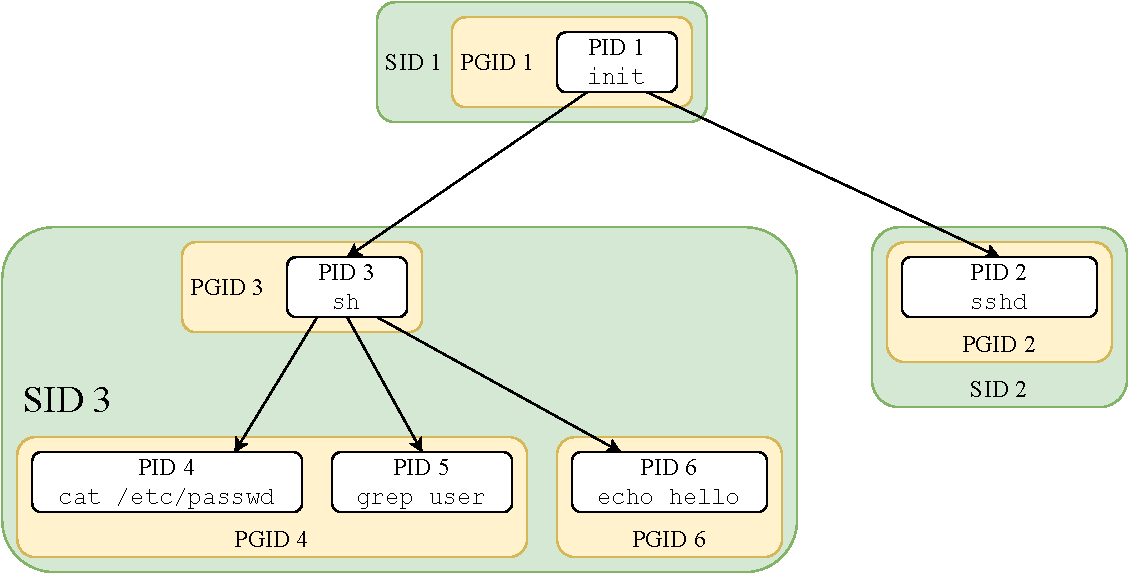
\includegraphics[width=\textwidth, keepaspectratio]{img/proc-hierarchy}
  \caption{A typical process hierarchy.}
  \label{fig:proc-hierarchy}
\end{figure}

\subsubsection{Orphaned process groups}

As we have just explained, processes belonging to the same shell job are put
inside the same process group. The shell is responsible for managing jobs, which
means keeping track of changes in their state (a job can become stopped when the
user inputs a special character), as well as manipulating them according to the
user's commands. However, when a shell exits, perhaps due to a bug, there might
no longer be a process managing these jobs. Specifically, there might no longer
be a process that can continue stopped jobs. Those jobs are doomed to being
stopped forever!

This is where the concept of \textit{orphaned process groups} comes into play. A
process group is orphaned when none of the processes in the group have a parent
that is in the same session, but in a different process group.

Consider the example of a shell: all jobs are in a different process group, but
in the same session as the shell. Therefore, as long the shell is alive, the
process groups of the jobs are not orphaned. However, when the shell process
terminates, all children of the shell are \textit{reparented}, i.e. some other
process becomes their parent, usually the \textit{init} process with PID 1. The
new parent is usually in a different session, so after reparenting the process
groups of the jobs are orphaned.

To solve the problem of jobs being stopped forever, when a process group becomes
orphaned, if the process group contains at least one stopped process, then every
process in the group is sent a \Verb{SIGHUP} signal followed by a
\Verb{SIGCONT}. The \Verb{SIGCONT} signal will resume stopped processes, and the
\Verb{SIGHUP} signal notifies the processes that they are now orphaned (it will
also most likely kill the processes, as that is the signal's default action).

Furthermore, processes in orphaned process groups cannot be stopped by
\textit{terminal stop signals}, i.e. \Verb{SIGTSTP}, \Verb{SIGTTOU} and
\Verb{SIGTTIN}. These signal are explained in Section~\ref{job-control-signals}.

\subsection{Process groups in the Mimiker kernel}

We will now describe the implementation of process groups in the Mimiker
kernel. First, we lay out the data structures used. After that, we will go over
how processes enter and exit process groups.

\subsubsection{Data structures}

\subsubsection*{\Verb{pgrp_t}}

The \Verb{pgrp_t} structure represents a single process group.

\begin{listing}[H]
\begin{minted}{c}
typedef struct pgrp {
  mtx_t pg_lock;
  TAILQ_ENTRY(pgrp) pg_hash;
  TAILQ_HEAD(, proc) pg_members;
  session_t *pg_session;
  int pg_jobc;
  pgid_t pg_id;
} pgrp_t;
\end{minted}
\caption{\href{https://mimiker.ii.uni.wroc.pl/source/xref/mimiker/include/sys/proc.h?r=8a7b07bf\#62}{\Verb{include/sys/proc.h}: definition of \Verb{pgrp_t}.}}
\label{lst:pgrp}
\end{listing}

The \Verb{pg_lock} mutex synchronizes concurrent accesses to the list of
members. The \Verb{pg_hash} field is a list entry used to link the structure
into the global hashtable used to lookup process groups by PGID. 

All processes that are members of the process group are on the \Verb{pg_members}
list. The list allows easy access, e.g. when a signal needs to be sent to all
members of the group.

The \Verb{TAILQ_ENTRY} and \Verb{TAILQ_HEAD} macros are part of Mimiker's
infrastructure for creating and manipulating linked list-like structures, a
\textit{tail queue} (which is what \Verb{TAILQ} stands for) being one example.
The infrastructure has been imported from FreeBSD, so the FreeBSD manual
page~\cite{tailq-man} provides a good overview of its usage.

\Verb{pg_session} is a pointer to the \Verb{session_t} structure representing
the session that this process group is a part of. Every process group is a part
of some session.

The \Verb{pg_jobc} field is a counter that tracks how many processes
\textit{qualify the group for job control}. We say that a process qualifies the
group for job control if and only if its parent is in a different process group
and in the same session. This way, when \Verb{pg_jobc} drops to zero, we know
that the process group has become orphaned.

The \Verb{pg_id} field is simply the numeric ID of the process group.

\subsubsection*{\Verb{proc_t::p_pgrp}}

The \Verb{p_pgrp} field of the process descriptor structure is a pointer to the
group that the process is a member of.

\subsubsection{Changing process groups}

Listing~\ref{lst:pgrp-enter} shows kernel code implementing the POSIX
\Verb{setpgid()} function. \Verb{p} is the process that is performing the system
call, \Verb{target} is the PID of the process whose process group is to be
changed, and \Verb{pgid} is the PGID of the process group to which the target
process is to be moved.

\begin{listing}[H]
\begin{minted}{c}
int pgrp_enter(proc_t *p, pid_t target, pgid_t pgid) {
@\llabel{f1}@  SCOPED_MTX_LOCK(all_proc_mtx);
  proc_t *targetp = proc_find_raw(target);

@\llabel{f2}@  if (targetp == NULL || !proc_is_alive(targetp) ||
      (targetp != p && targetp->p_parent != p))
    return ESRCH;
@\llabel{f3}@  if (targetp == targetp->p_pgrp->pg_session->s_leader)
    return EPERM;
@\llabel{f4}@  if (targetp->p_pgrp->pg_session != p->p_pgrp->pg_session)
    return EPERM;

  pgrp_t *pg = pgrp_lookup(pgid);

  /* Create new group if one does not exist. */
@\llabel{f5}@  if (pg == NULL) {
    /* New pgrp can only be created with PGID = PID of target process. */
    if (pgid != target)
      return EPERM;
    pg = pgrp_create(pgid);
    pg->pg_session = p->p_pgrp->pg_session;
    session_hold(pg->pg_session);
@\llabel{f6}@  } else if (pg->pg_session != p->p_pgrp->pg_session) {
    /* Target process group must be in the same session
     * as the calling process. */
    return EPERM;
  }

@\llabel{f7}@  return _pgrp_enter(targetp, pg);
}
\end{minted}
\caption{\href{https://mimiker.ii.uni.wroc.pl/source/xref/mimiker/sys/kern/proc.c?r=119d39cb\#391}{\Verb{sys/kern/proc.c}: definition of \Verb{pgrp_enter()}.}}
\label{lst:pgrp-enter}
\end{listing}

First, we \ref{f1} acquire the \Verb{all_proc_mtx}, which synchronizes accesses
to process-tree structures, such as process groups and sessions. Next, lines
\ref{f2}, \ref{f3} and \ref{f4} respectively perform the following checks:
\begin{itemize}
\item The target process must exist, be alive (i.e. executing normally or
  stopped), and it must either be a child of the calling process, or be the
  calling process itself.
\item The target process must not be a session leader.
\item The target process must be in the same session as the calling process.
\end{itemize}
We then \ref{f5} check whether the target process group exists. If it doesn't,
it is created, but only if the requested PGID matches the PID of the target
process. At \ref{f6} we perform yet another permission check. Finally, we call
\Verb{_pgrp_enter()} to perform the actual work of changing the process group of
the target process.

Now, let's see how a process group switch actually happens.
\begin{listing}[H]
\begin{minted}{c}
static int _pgrp_enter(proc_t *p, pgrp_t *target) {
  pgrp_t *old_pgrp = p->p_pgrp;

@\llabel{g1}@  if (old_pgrp == target)
    return 0;

@\llabel{g2}@  pgrp_jobc_enter(p, target);
  pgrp_jobc_leave(p, old_pgrp);

@\llabel{g3}@  WITH_MTX_LOCK(&old_pgrp->pg_lock) {
    WITH_MTX_LOCK(&target->pg_lock) {
      WITH_PROC_LOCK(p) {
@\llabel{g4}@        TAILQ_REMOVE(&old_pgrp->pg_members, p, p_pglist);
        TAILQ_INSERT_HEAD(&target->pg_members, p, p_pglist);
        p->p_pgrp = target;
      }
    }
  }

@\llabel{g5}@  if (TAILQ_EMPTY(&old_pgrp->pg_members))
    pgrp_remove(old_pgrp);

  return 0;
}
\end{minted}
\caption{\href{https://mimiker.ii.uni.wroc.pl/source/xref/mimiker/sys/kern/proc.c?r=119d39cb\#311}{\Verb{sys/kern/proc.c}: definition of \Verb{_pgrp_enter()}.}}
\label{lst:-pgrp-enter}
\end{listing}

We first \ref{g1} check whether we need to change groups at all. If we do, we
\ref{g2} adjust the \Verb{pg_jobc} counters of the old group, target group, as
well as the process groups of all children of the process. We will examine these
functions in a minute.

The process group switch must appear atomic. For this reason, it is necessary to
hold \Verb{all_proc_mtx}, both the old group and target group's lock, and the
process lock of the target process. We acquire the necessary locks at \ref{g3}.
\Verb{all_proc_mtx} is not acquired, since it is already held by the caller of
\Verb{_pgrp_enter()}.

When acquiring two locks of the same type (in this case process group locks),
one has to be very careful not to cause a \textit{deadlock} (see
Section~\ref{chap:locking-rules}). The usual way to ensure safety from deadlocks
is to establish an ordering on the locks, and whenever multiple locks need to be
acquired, make sure all required locks are acquired according to that ordering.
However, in this case deadlock can be avoided without specifying an order on
process group locks, by enforcing the following rule:
\begin{quote}
  In order to acquire multiple process group locks, a thread must already hold
  the \Verb{all_proc_mtx} lock.
\end{quote}
With this rule in force, it is impossible for two threads to concurrently
attempt to acquire multiple process group locks, since \Verb{all_proc_mtx} will
act as a serializer between them. The rule is a natural fit in this particular
situation for two reasons:
\begin{itemize}
  \item \Verb{_pgrp_enter()} is the only place in the whole kernel where there
    is a need to acquire multiple process group locks.
  \item The \Verb{all_proc_mtx} lock is already held everywhere
    \Verb{_pgrp_enter()} is called. Therefore, virtually no code changes had to
    be made in order to accomodate this rule.
\end{itemize}

At \ref{g4}, we are finally ready to make the switch. We remove the process from
the old group's list of members, add it to the target group's list, and change
the \Verb{p_pgrp} pointer. For more details about the \Verb{TAILQ_*} macros,
see~\cite{tailq-man}.

At the end, we \ref{g5} check whether the process was the last remaining process
in the old group. If so, the process group is removed.

\subsubsection{Orphaned process groups}

The \Verb{pg_jobc} counters need to be adjusted whenever a process leaves or
enters a process group. However, it is not sufficient to adjust only the counter
of the process group being entered or left. When a process leaves a process
group, the children of the process may no longer qualify their process group for
job control.

Figure~\ref{fig:orphan} illustrates a scenario in which a call to
\Verb{setpgid()} causes the process group of a child of the calling process to
become orphaned. For this reason, it is necessary to check whether the children
still qualify their process groups for job control whenever leaving or entering
a process group.

\begin{figure}[h]
  \centering
  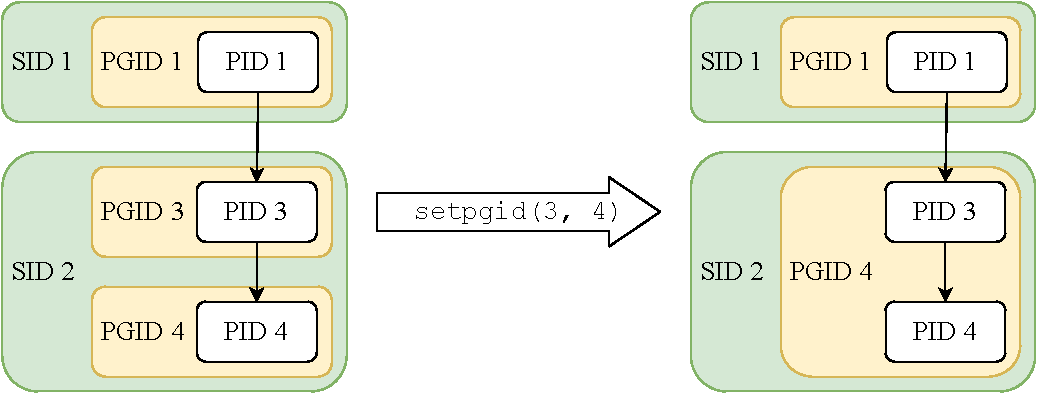
\includegraphics[width=\textwidth, keepaspectratio]{img/orphan}
  \caption{A parent's change of process group causes a child's process group to
    become orphaned.}
  \label{fig:orphan}
\end{figure}

The accounting associated with \Verb{pg_jobc} is split into two functions:\\
\Verb{pgrp_jobc_enter()} and \Verb{pgrp_jobc_leave()}.

\begin{listing}[H]
\begin{minted}{c}
static void pgrp_jobc_enter(proc_t *p, pgrp_t *pg) {
  assert(mtx_owned(all_proc_mtx));

@\llabel{h1}@  if (same_session_p(p->p_parent->p_pgrp, pg))
    pg->pg_jobc++;

  proc_t *child;
@\llabel{h2}@  TAILQ_FOREACH (child, CHILDREN(p), p_child)
    if (same_session_p(child->p_pgrp, pg))
      child->p_pgrp->pg_jobc++;
}
\end{minted}
\caption{\href{https://mimiker.ii.uni.wroc.pl/source/xref/mimiker/sys/kern/proc.c?r=119d39cb\#239}{\Verb{sys/kern/proc.c}: definition of \Verb{pgrp_jobc_enter()}.}}
\label{lst:-pgrp-enter}
\end{listing}

\Verb{p} is the process entering the process group \Verb{pg}.
The \Verb{same_session_p()} function returns \Verb{true} if and only if the two
groups are different, but in the same session.

At \ref{h1}, we check whether \Verb{p} will qualify the process group \Verb{pg}
for job control after entering it. If so, the \Verb{pg_jobc} counter is
incremented.

Next, at \ref{h2} we do the same for the children of \Verb{p}: we check whether
they will qualify their process groups after \Verb{p} enters \Verb{pg}. If so,
the group's \Verb{pg_jobc} is incremented.

The \Verb{pgrp_jobc_leave()} function has a very similar structure, except now
we call \Verb{pgrp_maybe_orphan()} instead of incrementing \Verb{pg_jobc}. The
\Verb{pgrp_maybe_orphan()} function decrements the process group's
\Verb{pg_jobc}, and if it reaches zero, sends the appropriate signals.

\begin{listing}[H]
\begin{minted}{c}
static void pgrp_jobc_leave(proc_t *p, pgrp_t *pg) {
  assert(mtx_owned(all_proc_mtx));

  if (same_session_p(p->p_parent->p_pgrp, pg))
    pgrp_maybe_orphan(pg);

  proc_t *child;
  TAILQ_FOREACH (child, CHILDREN(p), p_child)
    if (same_session_p(child->p_pgrp, pg))
      pgrp_maybe_orphan(child->p_pgrp);
}
\end{minted}
\caption{\href{https://mimiker.ii.uni.wroc.pl/source/xref/mimiker/sys/kern/proc.c?r=119d39cb\#251}{\Verb{sys/kern/proc.c}: definition of \Verb{pgrp_jobc_leave()}.}}
\label{lst:-pgrp-enter}
\end{listing}

\subsection{Sessions in the Mimiker kernel}
\label{chap:sessions}

We will now examine the implementation of sessions in the Mimiker kernel. After
looking at the session data structure, we will see how new sessions are created.

\subsubsection{Data structures}

The \Verb{session_t} data structure represents a single session.
Listing~\ref{lst:sess} presents its complete definition.

\begin{listing}[H]
\begin{minted}{c}
typedef struct session {
  TAILQ_ENTRY(session) s_hash;
  proc_t *s_leader;
  int s_count;
  sid_t s_sid;
  tty_t *s_tty;
  char s_login[LOGIN_NAME_MAX];
} session_t;
\end{minted}
\caption{\href{https://mimiker.ii.uni.wroc.pl/source/xref/mimiker/include/sys/proc.h?r=8a7b07bf\#42}{\Verb{include/sys/proc.h}: definition of \Verb{session_t}.}}
\label{lst:sess}
\end{listing}

The \Verb{s_hash} field is used to link the structure into the hashtable used to
look up session strucutures by their session ID (SID).

The \Verb{s_leader} field points to the process that is the session leader, i.e.
the process that created the session by calling the \Verb{setsid()} function.
Once the session leader terminates, the \Verb{s_leader} field of the session is
set to \Verb{NULL}.

The \Verb{s_count} field counts the number of process groups belonging to the
session. Whenever a new process group joins the session, the
\Verb{session_hold()} function increments the \Verb{s_count} field (see
Listing~\ref{lst:pgrp-enter} for an example of its usage). When a process group
is removed, the \Verb{pgrp_remove()} function, which can be seen used in
Listing~\ref{lst:-pgrp-enter} decrements the session's \Verb{s_count} field.
Once the value of the field reaches zero, the session is removed from the kernel
and the memory occupied by the structure is reclaimed.

The \Verb{s_sid} field holds the numeric ID of the session. It is equal to the
PID of the process that created the session.

The \Verb{s_tty} field is a pointer to the session's controlling terminal. For
interactive sessions (i.e. sessions created by a user logging into the system
and launching a shell), the controlling terminal is the device that provides
input to the shell and spawned jobs, and receives their output. Not every
session has a controlling terminal: daemon processes are usually placed in
sessions without a controlling terminal. If a session has no controlling
terminal, the value of its \Verb{s_tty} field is set to \Verb{NULL}.

\subsubsection{Creating a session}

User processes can create new sessions using the \Verb{setsid()} function from
the C library. That function directly calls the \Verb{setsid()} system call,
which is implemented by the \Verb{sys_setsid()} function in the kernel. That
function, in turn, calls \Verb{session_enter()} to do the work.
Listing~\ref{lst:session-enter} presents the source code of
\Verb{session_enter()}.

\begin{listing}[H]
\begin{minted}{c}
int session_enter(proc_t *p) {
@\llabel{i1}@  SCOPED_MTX_LOCK(&all_proc_mtx);

  pgid_t pgid = p->p_pid;
  pgrp_t *pg = pgrp_lookup(pgid);

@\llabel{i2}@  if (pg)
    return EPERM;

@\llabel{i3}@  pg = pgrp_create(pgid);
@\llabel{i4}@  pg->pg_session = session_create(p);

@\llabel{i5}@  return _pgrp_enter(p, pg);
}
\end{minted}
\caption{\href{https://mimiker.ii.uni.wroc.pl/source/xref/mimiker/sys/kern/proc.c?r=119d39cb\#341}{\Verb{sys/kern/proc.c}: definition of \Verb{session_enter()}.}}
\label{lst:session-enter}
\end{listing}

First, we \ref{i1} acquire the \Verb{all_proc_mtx} lock, which is required to perform
things such as process group lookups and creating new sessions and process
groups.

At \ref{i2}, we ensure that there doesn't already exist a process group with the
same PGID as the PID of the calling process. The process group that is created as
a result of creating a new session has a PGID equal to the PID of the calling
process, and if a group with such a PGID already exists, we can't create the
group we need, since PGIDs must be unique.

Once we have ensured that we can create the group, we do so at \ref{i3}. Then,
we \ref{i4} create a new session with \Verb{p} as the session leader and link it
to the newly created group (the session created by \Verb{session_create()} has a
\Verb{s_count} of 1, so there's no need to adjust it). Finally, we \ref{i5}
change the process group of the calling process to the one we just created.

\section{Job Control Signals}

\subsection{POSIX signals}\label{chap:signals}

\textit{Signals} are used to notify processes of various events. These events
can occur \textit{synchronously} or \textit{asynchronously} with respect to the
process receiving the signal. POSIX signal semantics are (intentionally) very
similar to those found in the original UNIX operating system
\cite[Section~7.2]{unix-book}.

A \textit{synchronous signal} is sent as a direct consequence of some (usually
erroneous) action being performed by the receiving process. For instance, a
process is sent a \Verb{SIGSEGV} signal upon trying to access an invalid
memory location.

An \textit{asynchronous signal} is sent independently of the actions of the
receiving process, and may be received at any time. For example, whenever a
process terminates, the system sends a \Verb{SIGCHLD} signal to its parent.

Signals can be sent by the operating system in response to certain events (e.g.
process termination), or by other processes, using the \Verb{kill()} function
\cite{kill}. A process can send a signal to itself using the \Verb{raise()}
function. As a shorthand, we shall say that a signal is sent to a process
group when it's sent to every process that is a member of the group.

The type of signal (\Verb{SIGSEGV}, \Verb{SIGCHLD}, etc.) is determined by
the \textit{signal number}. In fact, \Verb{SIGSEGV} and others are \textit{C
  preprocessor macros} that expand to unique signal numbers.

Processes can take different actions in response to signals with different
numbers. Every process has its own set of \textit{signal actions} associated
with every signal number. The action associated with a signal is also called its
\textit{disposition}. There are three possible actions that can be taken in
response to a signal:
\begin{enumerate}
\item Take the default action for that signal number.
  
  Every signal number has an associated default action. For instance, the
  default action of the \Verb{SIGSEGV} signal is to immediately terminate the
  receiving process.
\item Ignore the signal.
\item Invoke a \textit{signal handler routine}.

  The handler routine is run in the context of the process that receiving
  process. After the handler finishes execution, the process is resumed.
\end{enumerate}

The mapping of signal numbers to signal actions is controlled using the
\Verb{sigaction()} function \cite{sigaction}. Not every signal can have its
action modified: \Verb{SIGKILL} and \Verb{SIGSTOP} cannot have their actions
changed from the default one, which is to terminate or stop the receiving process,
respectively.

The \textit{delivery} of a signal occurs when the target (i.e. receiving)
process takes the action associated with the signal. A signal may be delivered
long after it is initially sent, or it may not be delivered at all, even if it
isn't ignored. This is because a process may \textit{block} a set of signals
from being delivered. A blocked signal cannot be delivered until it is
unblocked. Contrary to signals that are ignored, blocked signals await delivery
instead of being discarded.

The \textit{signal mask} determines the set of blocked signals for a thread. It
can be examined and modified using the \Verb{sigprocmask()} function
\cite{sigprocmask}. Unsurprisingly, the \Verb{SIGKILL} and \Verb{SIGSTOP}
signals cannot be blocked from being delivered.

\subsection{Signals used for job control}
\label{job-control-signals}

The following signals are most commonly used to control jobs on POSIX-compliant
operating systems:
\begin{itemize}
\item \Verb{SIGINT}

  Sent by the operating system in response to the special character \Verb{VINTR}
  (which commonly corresponds to \Verb{^C}, i.e. Control-C) being received on
  the terminal. Its purpose is to signal interruption by the user. A process
  that receives this signal is usually expected to terminate shortly. The
  default action associated with this signal is to terminate the receiving
  process.

\item \Verb{SIGQUIT}

  Similar to \Verb{SIGINT}, except it is sent in response to the \Verb{VQUIT}
  character (usually~\Verb{^\}), and the default action additionally generates
  a core dump of the receiving process.

\item \Verb{SIGTTOU}

  Sent by the operating system whenever a background job attempts to write to
  the terminal, provided the \Verb{TOSTOP} terminal flag is set (we will say
  more about terminal flags later). The default action associated with this
  signal is to stop the receiving process.
  
\item \Verb{SIGTTIN}

  Sent by the operating system whenever a background job attempts to read from
  the terminal. Background jobs may not read from the terminal, regardless of
  the terminal settings. The default action associated with this signal is to
  stop the receiving process.

\item \Verb{SIGTSTP}

  Sent by the operating system in response to the special character \Verb{VSUSP}
  (usually~\Verb{^Z}) being received on the terminal. Its purpose is to stop the
  foreground job. Well-behaving processes should not ignore this signal. Many
  programs need to do some cleanup before stopping: in that case, they register
  a handler that does the necessary cleanup, after which it performs
  \Verb{raise(SIGSTOP)}. The default action associated with this signal is to
  stop the receiving process.

\item \Verb{SIGSTOP}

  This signal is not sent by the operating system. It unconditionally stops the
  receiving process. It cannot be blocked or ignored. 

\item \Verb{SIGCONT}

  This is the only signal that can resume a stopped process (apart from
  \Verb{SIGKILL}, which resumes it only to immediately terminate it). It is
  usually sent by the shell, e.g.\ when a background job that was stopped by a
  \Verb{SIGTTIN} signal is brought into the foreground.

\item \Verb{SIGCHLD}

  Sent by the operating system in response to the termination of a process. The
  signal is sent to the parent of the terminating process. Shells use this
  signal to update their data on currently running jobs.
\end{itemize}

\subsection{Signals in the Mimiker kernel}

In this subsection we describe the implementation of signals in the Mimiker
kernel. First, we lay out the data structures used, after which we go through
how exactly signals are sent and delivered in the kernel. Lastly, we examine how
processes are stopped in response to the delivery of a stop signal.

\subsubsection{Signal data structures}

We will now describe the various data types and structures that are critical to
the implementation of signals in the Mimiker kernel.

\subsubsection*{\Verb{sigaction_t}}


The \Verb{sigaction_t} data type describes the disposition of a signal.
\begin{listing}[H]
\begin{minted}{c}
typedef void (*sig_t)(int); /* type of signal function */

typedef struct sigaction {
  union {
    sig_t sa_handler;
    void (*sa_sigaction)(int, siginfo_t *, void *);
  };
  sigset_t sa_mask;
  int sa_flags;
} sigaction_t;
\end{minted}
\caption{\href{https://mimiker.ii.uni.wroc.pl/source/xref/mimiker/include/sys/signal.h?r=225c20cd\#41}{\Verb{include/sys/signal.h}: definition of \Verb{sigaction_t}.}}
\end{listing}

The \Verb{sa_handler} and \Verb{sa_sigaction} fields are
simply pointers to a signal handler function. Processes can register either a
handler of type \Verb{sig_t}, which takes only the signal number as an
argument, or a handler that takes two additional arguments:
\begin{itemize}
\item A pointer to a structure of type \Verb{siginfo_t}, which contains
  more information about the signal (e.g.\ in the case of
  \Verb{SIGCHLD}, the PID of the child process).

\item A pointer that can be cast to a pointer to a structure of type
  \Verb{ucontext_t}, which holds the processor context of the thread
  that received the signal at the time of the signal's delivery.
\end{itemize}
The \Verb{sa_handler} field can also have the special value
\Verb{SIG_DFL} or \Verb{SIG_IGN}, which respectively mean
that the signal has the default disposition or is ignored.

The \Verb{sa_mask} field is the set of signals that are blocked
during the execution of the handler function. After the handler finishes, the
signal mask is restored to its previous state.
 
The \Verb{sa_flags} field is a set of flags that modify the behaviour
of the signal in various ways. At the time of writing, the only flag supported
in the Mimiker kernel is \Verb{SA_RESTART}, which causes system calls
that are interrupted by a signal handler to be automatically restarted,
transparently to the process that issued the system call.

\subsubsection*{\Verb{proc_t::p_sigactions}}

The \Verb{p_sigactions} field of the \Verb{proc_t} (i.e.
process descriptor) structure is an array of structures of type
\Verb{sigaction_t}. For each signal number \Verb{signo}, the
disposition of that signal for the process is stored in
\Verb{p_sigactions[signo]}.

\subsubsection*{\Verb{thread_t::td_sigmask}}

As opposed to the signal disposition, which is shared by all the threads of a
process, every thread has its own set of blocked signals. This set is stored in
the \Verb{td_sigmask} field of the \Verb{thread_t} structure,
which describes a single thread of execution. The field is just a bit vector,
with each bit corresponding to a signal number. If a bit is set, signals with
the corresponding number are blocked from being delivered.

\subsubsection*{\Verb{thread_t::td_sigpend}}

The \Verb{td_sigpend} field of the \Verb{thread_t} structure
represents pending signals, i.e.\ signals that have been sent to the thread and
are waiting to be delivered. It is a structure of type
\Verb{sigpend_t}, which consists of a bit vector of pending signal
numbers, as well as a list of \Verb{ksiginfo_t} structures which carry
additional information about signals.

\subsubsection{Sending a signal}

We will now walk through the code that does the actual work of sending a signal
to a process. Sending signals in the Mimiker kernel is accomplished using the
\Verb{sig_kill()} function. Listing~\ref{lst:sig-kill} contains slightly
simplified code of the function.

\begin{listing}[H]
\begin{minted}{c}
void sig_kill(proc_t *p, ksiginfo_t *ksi) {
@\llabel{a1}@  assert(mtx_owned(&p->p_lock));

  signo_t sig = ksi->ksi_signo;
  thread_t *td = p->p_thread;
  bool ignored = sig_ignored(p->p_sigactions, sig);

@\llabel{a2}@  if ((ignored && !sigprop_cont(sig)) || sig_ignore_ttystop(p, sig))
    return;

  /* If sending a stop or continue signal,
   * remove pending signals with the opposite effect. */
@\llabel{a3}@  if (defact_stop(sig)) {
    sigpend_get(&td->td_sigpend, SIGCONT, NULL);
  } else if (sigprop_cont(sig)) {
    sigpend_delete_set(&td->td_sigpend, &stopmask);
@\llabel{a4}@    if (p->p_state == PS_STOPPED)
      proc_continue(p);
    if (ignored)
      return;
  }

@\llabel{a5}@  sigpend_put(&td->td_sigpend, ksiginfo_copy(ksi));

@\llabel{a6}@  if (__sigismember(&td->td_sigmask, sig))
    return;

  WITH_SPIN_LOCK (td->td_lock) {
@\llabel{a7}@    td->td_flags |= TDF_NEEDSIGCHK;
    if (td_is_interruptible(td)) {
      spin_unlock(td->td_lock);
@\llabel{a8}@      sleepq_abort(td); /* Locks & unlocks td_lock */
      spin_lock(td->td_lock);
    }
  }
}
\end{minted}
\caption{\href{https://mimiker.ii.uni.wroc.pl/source/xref/mimiker/sys/kern/signal.c?r=97a49381\#351}{\Verb{sys/kern/signal.c}: definition of \Verb{sig_kill()}.}}
\label{lst:sig-kill}
\end{listing}

The function accepts two parameters. The first is a pointer to a \Verb{proc_t}
structure, which represents the process that the signal will be sent to. The
second is a pointer to a \Verb{ksiginfo_t} structure, which describes the signal
to be sent. Most importantly, it contains the signal number.

The assertion at \ref{a1} ensures that the function's caller has acquired the
necessary lock. Processes' and threads' signal data structures are globally
shared (i.e. many threads of execution can access them), so access to them must
be synchronized using locks.

We then \ref{a2} quickly filter out ignored signals, with an exception for
signals that can resume stopped processes, as these signals have an effect on
the target process (i.e. continue it) even if they are ignored. Furthermore,
terminal stop signals (\Verb{SIGTSTP}, \Verb{SIGTTOU} and \Verb{SIGTTIN}) cannot
stop a process which is in an orphaned process group: this case is detected by
the \Verb{sig_ignore_ttystop()} function.

In \ref{a3}, we check whether the signal being sent is a stop or continue
signal. If it is, we remove all signals that are already pending which have the
opposite effect. Additionally, for continue signals \ref{a4} we check whether
the target process is stopped. If it is, we wake it up and notify its parent.

Once control reaches \ref{a5}, we are certain that the signal isn't ignored, so
it should be queued for delivery to the target process. The \Verb{sigpend_put}
function inserts the signal into the set of pending signals for the target
process's thread.

The final step is notifying the thread that it needs to process its pending
signals. This step is skipped if \ref{a6} the signal is blocked from being
delivered. The \ref{a7} \Verb{TDF_NEEDSIGCHK} flag lets the thread know that it
should check for pending signals at the nearest opportunity. If the thread is
\textit{sleeping interruptibly} (e.g. blocked inside a \Verb{read()} call on a
terminal device, awaiting user input), it is \ref{a8} awakened so that it can
receive the signal. The need to release \Verb{td_lock} before calling
\Verb{sleepq_abort()} is an unfortunate consequence of \textit{lock ordering},
as the function acquires another spinlock before acquiring \Verb{td_lock}.
Section~\ref{chap:locking-rules} goes into more detail about lock ordering.


\subsubsection{Signal delivery}

After a signal is sent, it remains in the pending set, waiting to be delivered.
Signals are delivered to a process whenever control is transferred from the
kernel to that process, i.e. on transitions from the kernel to userspace. Every
time before returning to userspace, either from executing a system call, or
handling an interrupt or exception that occurred while the CPU was executing
userspace code, the \Verb{on_user_exc_leave()} function is called. This function
handles signal delivery and system call restarting.

\begin{listing}[H]
\begin{minted}{c}
void on_user_exc_leave(mcontext_t *ctx, syscall_result_t *result) {
  thread_t *td = thread_self();
  proc_t *p = td->td_proc;
  int sig = 0;
  ksiginfo_t ksi;

@\llabel{q0}@  if (td->td_flags & TDF_NEEDSIGCHK) {
    WITH_PROC_LOCK(p) {
@\llabel{q1}@      sig = sig_check(td, &ksi);
    }
  }

  if (result)
@\llabel{q2}@    set_syscall_retval(ctx, result, sig);

@\llabel{q3}@  while (sig) {
    WITH_PROC_LOCK(p) {
@\llabel{q4}@      sig_post(&ksi);
@\llabel{q5}@      sig = sig_check(td, &ksi);
    }
  }
}
\end{minted}
\caption{\href{https://mimiker.ii.uni.wroc.pl/source/xref/mimiker/sys/kern/exception.c?r=4cae32de\#57}{\Verb{sys/kern/exception.c}: definition of \Verb{on_user_exc_leave()}.}}
\label{lst:on-user-exc-leave}
\end{listing}

Signal delivery can be divided into two steps: checking for a pending signal,
and \textit{posting} a signal found to be pending. Posting a signal means
setting up the execution context of the process, so that the signal handler is
the first thing that is executed after returning control to the process.

The first step is therefore to check for pending signals. The
\Verb{TDF_NEEDSIGCHK} flag indicates that a signal is pending. It is set in
\Verb{sig_kill()}, see Listing~\ref{lst:sig-kill}. We check the flag at \ref{q0}
to avoid unnecessarily acquiring the process lock and checking the set of
pending signals. If the flag is set, we \ref{q1} call \Verb{sig_check()}, which
returns the signal number of a signal that needs to be posted, or \Verb{0} if no
signal needs posting. Note that signals with special effects (i.e.\ stopping or
killing a process) are not posted, but are instead handled inside
\Verb{sig_check()}, as part of checking for a pending signal. This is an
implementation choice that simplifies handling of certain edge cases.

Before posting pending signals, we \ref{q2} set the return value of the system
call we're returning from using \Verb{set_syscall_retval()} (provided we're
returning from a system call at all). Note that \Verb{on_user_exc_leave()} is
also called when returning to userspace from an interrupt, in which case
\Verb{result} is set \Verb{NULL} to indicate that we're not returning from a
system call. The \Verb{set_syscall_retval()} function also restarts the system
call if needed. More details about system call restarting are given in
Section~\ref{chap:sleep-stop}.

The last step is to post all pending signals. We \ref{q3} loop as long as there
is a signal that needs posting. Inside the loop, the currently selected signal
is \ref{q4} posted and \ref{q5} another signal is selected. We will not describe
how signals are posted, as most of the details are architecture-specific, and we
are primarily concerned with job control signals, which are not posted at all
(unless they have registered handlers, in which case they don't behave like job
control signals).

The control flow inside \Verb{on_user_exc_leave()} may seem confusing, but there
is a reason for it. The main issue is that \Verb{set_syscall_retval()} must know
whether a signal will be posted (note \Verb{sig} being passed as an argument to
it), but it must also be called \textit{before} \Verb{sig_post()}. The reason is
that \Verb{set_syscall_retval()} modifies the context of the userspace thread
that invoked the system call, and \Verb{sig_post()} also modifies the context to
arrange for the signal handler to be called. The modifications made by
\Verb{set_syscall_retval()} must precede the ones made by \Verb{sig_post()},
hence the somewhat convoluted control flow.

Let us now focus on the \Verb{sig_check()} function, which checks for pending
signals and handles job control signals. Listing~\ref{lst:sig-check} contains
the source code of the function.

\begin{listing}[H]
\begin{minted}{c}
int sig_check(thread_t *td, ksiginfo_t *out) {
  proc_t *p = td->td_proc;
  signo_t sig;

@\llabel{b0}@  assert(mtx_owned(&p->p_lock));

@\llabel{b1}@  while ((sig = sig_pending(td))) {
@\llabel{b2}@    sigpend_get(&td->td_sigpend, sig, out);

@\llabel{b3}@    if (sig_should_stop(p->p_sigactions, sig)) {
      if (!sig_ignore_ttystop(p, sig))
        proc_stop(sig);
      continue;
    }

@\llabel{b4}@    if (sig_should_kill(p->p_sigactions, sig))
      sig_exit(td, sig);

@\llabel{b5}@    return sig;
  }

  WITH_SPIN_LOCK (td->td_lock)
@\llabel{b6}@    td->td_flags &= ~TDF_NEEDSIGCHK;
@\llabel{b7}@  return 0;
}
\end{minted}
\caption{\href{https://mimiker.ii.uni.wroc.pl/source/xref/mimiker/sys/kern/signal.c?r=97a49381\#454}{\Verb{sys/kern/signal.c}: definition of \Verb{sig_check()}.}}
\label{lst:sig-check}
\end{listing}

This function manipulates signal state, which is protected by the process's
lock, hence the assertion at \ref{b0}.

The function first \ref{b1} extracts a pending signal that is not currently
blocked using the \Verb{sig_pending()} function. It returns just a signal
number, so in the next step \ref{b2} we remove the signal from the set of
pending signals.

We then check \ref{b3} if the signal should stop the receiving process. Notice
that after the process is stopped using \Verb{proc_stop()} and subsequently
resumed by another process, control goes back to \ref{b1}.

Next, we \ref{b4} handle signals that should kill the process. The
\Verb{sig_exit()} function terminates the calling process and never returns.

If the pending signal is neither a stop nor a kill signal, \ref{b5} the signal
number is returned. Additional information about the signal is passed to the
caller via the \Verb{out} output parameter. The signal is then passed to
\Verb{sig_post()} to arrange for the handler to be called.

If no signal needs to be posted, the function \ref{b6} clears the thread's
\Verb{TDF_NEEDSIGCHK} flag, since there is no need to check for pending signals
anymore. A return value of 0 \ref{b7} indicates to the caller that no signal
needs to be posted.

\subsubsection{Stopping and continuing processes}

One of the job control features that were implemented from scratch as part of
the implementation effort described in this thesis is support for stopping and
continuing processes by means of the \Verb{SIGSTOP} and \Verb{SIGCONT} signals.

A process is always in one of several states, denoted by the value of the
\Verb{p_state} field in the process descriptor. When a process is executing
normally, its state is \Verb{PS_NORMAL}. When a process is stopped, its state is
\Verb{PS_STOPPED}. All the threads of a stopped process are also stopped and
unable to run until the process is continued.

The \Verb{proc_stop()} function stops the current process in response to a stop
signal. Its source code is listed in Listing~\ref{lst:proc-stop}.

\begin{listing}[H]
\begin{minted}{c}
void proc_stop(signo_t sig) {
  thread_t *td = thread_self();
  proc_t *p = td->td_proc;

@\llabel{c1}@ assert(mtx_owned(&p->p_lock));
  assert(p->p_state == PS_NORMAL);

@\llabel{c2}@  p->p_state = PS_STOPPED;
@\llabel{c3}@  p->p_stopsig = sig;
  p->p_flags |= PF_STATE_CHANGED;
  WITH_PROC_LOCK(p->p_parent) {
@\llabel{c4}@    proc_wakeup_parent(p->p_parent);
    sig_child(p, CLD_STOPPED);
  }
@\llabel{c5}@  WITH_SPIN_LOCK (td->td_lock) { td->td_flags |= TDF_STOPPING; }
  proc_unlock(p);
  /* We're holding no locks here, so our process can be continued before we
   * actually stop the thread. This is why we need the TDF_STOPPING flag. */
  spin_lock(td->td_lock);
@\llabel{c6}@  if (td->td_flags & TDF_STOPPING) {
    td->td_flags &= ~TDF_STOPPING;
    td->td_state = TDS_STOPPED;
@\llabel{c7}@    sched_switch(); /* Releases td_lock. */
  } else {
    spin_unlock(td->td_lock);
  }
  proc_lock(p);
  return;
}
\end{minted}
\caption{\href{https://mimiker.ii.uni.wroc.pl/source/xref/mimiker/sys/kern/proc.c?r=119d39cb\#823}{\Verb{sys/kern/proc.c}: definition of \Verb{proc_stop()}.}}
\label{lst:proc-stop}
\end{listing}

This function manipulates process state, hence the assertion at \ref{c1}. The
next assertion simply makes sure that the process is in the expected state.
Next, at \ref{c2} the process state is set to \Verb{PS_STOPPED}.

At \ref{c3}, we set up information that is used by the \Verb{wait4()} system
call. It is used by a process to wait for one of its children to change state.
As the reader might have already guessed, stopping counts as a state change. The
call to \Verb{proc_wakeup_parent()} at \ref{c4} notifies the parent process of
the status change. In the next line, a \Verb{SIGCHLD} signal is sent to the
parent.

The rest of the function attempts to stop the process's thread. This task is
fairly simple, due to the fact that all processes in the Mimiker kernel are
single-threaded. Still, it is not as simple as one might like, due to some
technicalities around locking.

Specifically, we are not allowed to hold the current thread's spinlock (in this
case, \Verb{td->td_lock}) while releasing a mutex. This restriction does not
apply to any other spinlocks, which can be held while releasing a mutex.
Furthermore, we must release the process's lock before stopping the thread in
\Verb{sched_switch()}, and the thread's spinlock must be held when calling
\Verb{sched_switch()}. These constraints require us to briefly hold no locks at
all. During this window of time, another process might continue the process we
are trying to stop, in which case we should not stop the thread.

The solution is to add the \Verb{TDF_STOPPING} thread flag, which signals that
the thread is about to stop, but hasn't stopped yet. It is set \ref{c5} while
still holding the process's lock. If the process is continued before the thread
is stopped, the \Verb{TDF_STOPPING} flag is cleared. The stopping thread
examines \ref{c6} the flag before changing its state. Thanks to this, the thread
will stop only if the process is still stopped.

After setting the thread state to \Verb{TDS_STOPPED}, the call \ref{c7} to
\Verb{sched_switch()} hands over control to the scheduler, which will select
another thread to run. The stopped thread will not be selected by the scheduler
to run until it is continued.

Let us now see how stopped processes are woken up. Continuing a process is
simpler than stopping one, as can be seen by looking at
Listing~\ref{lst:proc-continue}.

\begin{listing}[H]
\begin{minted}{c}
void proc_continue(proc_t *p) {
  thread_t *td = p->p_thread;

@\llabel{d1}@  assert(mtx_owned(&p->p_lock));
  assert(p->p_state == PS_STOPPED);

@\llabel{d2}@  p->p_state = PS_NORMAL;
@\llabel{d3}@  p->p_flags |= PF_STATE_CHANGED;
  WITH_PROC_LOCK(p->p_parent) {
    proc_wakeup_parent(p->p_parent);
  }
@\llabel{d4}@  WITH_SPIN_LOCK (td->td_lock) { thread_continue(td); }
}
\end{minted}
\caption{\href{https://mimiker.ii.uni.wroc.pl/source/xref/mimiker/sys/kern/proc.c?r=119d39cb\#854}{\Verb{sys/kern/proc.c}: definition of \Verb{proc_continue()}.}}
\label{lst:proc-continue}
\end{listing}

The assertion at \ref{d1} should come as no surprise at this point, as we are
modifying the process's state. The next assertion ensures that we only attempt
to continue processes that are actually stopped.

We then \ref{d2} restore the process's \Verb{p_state} to \Verb{PS_NORMAL}. Next,
we \ref{d3} notify the parent of the state change. Note that, in contrast to
\Verb{proc_stop()}, we don't send a \Verb{SIGCHLD} signal to the parent process.
This is in line with the POSIX specification.

Lastly, we \ref{d4} wake up the thread of the process we are continuing. The
\Verb{thread_continue()} function is very simple, and is presented in
Listing~\ref{lst:thread-continue}.

\begin{listing}[H]
\begin{minted}{c}
void thread_continue(thread_t *td) {
@\llabel{e1}@  if (td->td_flags & TDF_STOPPING) {
    td->td_flags &= ~TDF_STOPPING;
  } else {
@\llabel{e2}@    assert(td_is_stopped(td));
@\llabel{e3}@    sched_wakeup(td, 0);
  }
}
\end{minted}
\caption{\href{https://mimiker.ii.uni.wroc.pl/source/xref/mimiker/sys/kern/thread.c?r=27b8c19a\#210}{\Verb{sys/kern/thread.c}: definition of \Verb{thread_continue()}.}}
\label{lst:thread-continue}
\end{listing}

An important thing to notice is that even if a process's state indicates that it
is stopped (i.e. \Verb{p_state == PS_STOPPED}), its thread is not guaranteed to
also be stopped (i.e. \Verb{td_state == TDS_STOPPED}). The call to
\Verb{proc_continue()} can occur at the time in \Verb{proc_stop()} where we are
not holding any locks.

For this reason, we first \ref{e1} check the \Verb{TDF_STOPPING} flag. If it is
set, the thread has not stopped yet, and all we need to do is clear the flag.
If the flag is not set, then we know that the thread is stopped, hence the
assertion at \ref{e2}. We then \ref{e3} call \Verb{sched_wakeup()} to make the
thread runnable again.

\chapter{The Terminal Subsystem}\label{chap:tty}

The implementation of the terminal subsystem in the Mimiker kernel consists of
three primary components:
\begin{itemize}
\item The device-independent terminal layer.
\item The UART terminal driver.
\item The \textit{pseudoterminal} subsystem, which includes another terminal
  driver.
\end{itemize}

In this chapter, we will describe each component in detail. Before describing
the implementation, we will present relevant parts of the POSIX specification.

This chapter uses concepts such as \textit{terminals}, \textit{terminal
  devices}, and \textit{terminal drivers}. Their meanings are as follows:
\begin{itemize}
\item A \textit{terminal} does \textbf{not} refer to a hardware device like a
  teletype. Instead, it is an abstract representation of such a device in the
  kernel, not tied to a specific hardware model. In fact, it may not even be
  ``backed'' by any actual hardware device, thanks to pseudoterminals. The
  terminal layer implements the device-independent functions of a terminal.
\item A \textit{terminal device} is the hardware device that can be represented
  by an abstract terminal. A UART is an example of a terminal device.
\item A \textit{terminal driver} acts as the ``glue'' between the terminal layer
  (which is device-independent) and a specific hardware device.
\end{itemize}

\section{The terminal layer}

The terminal layer provides a layer of processing between processes and the
terminal device. This processing might seem unnecessary at first, but its
usefulness very quickly becomes apparent.

For example, on UNIX-like systems a long-running command can be interrupted by
pressing the Control-C combination of keys on the keyboard. If there was no
processing done on incoming characters by the operating system, the process in
question would simply receive the character as input, and it would be up to the
process to respond to it. The process would need to be prepared to receive such
characters at any time. This is clearly an inconvenience, especially for simple
programs.

With the processing done by the operating system, the behavior is uniform and
requires less effort from writers of userspace programs. The interruption is
delivered as a signal, for which a handler can be easily installed.

The preceding example illustrates just one useful feature of terminals. 
The POSIX specification includes the concept of terminals, and describes how
incoming and outgoing characters should be processed by the terminal subsystem. 
We will now present the most important aspects of this specification.

% While physical terminal devices are no longer in common use, many users of
% UNIX-like prefer to use the command line for certain tasks. The command line, or
% more precisely, the \textit{shell}, makes use of certain feature

A very detailed description of the terminal interfaces available in several
UNIX-like operating systems, which goes well beyond POSIX, is presented in
\cite[Chapter~18]{apue}. For a Linux-specific discussion, see
\cite[Chapter~62]{tlpi}.

\subsection{POSIX terminals}\label{chap:posix-terminals}

On the surface, a terminal is no different than a standard character device. To
interact with it, a process can open the corresponding device file using
\Verb{open()} and then perform input and output using \Verb{read()} and
\Verb{write()} respectively. The terminal interface specified by POSIX is much
richer than that. Terminals play a significant role in job control, and
therefore are connected to the concepts of process groups and sessions. We will
now examine the most important aspects of the terminal specification
\cite{terminal-spec} found in POSIX and see how terminals tie into job control.

\subsubsection{Terminal input and output}

Data coming in from the hardware terminal device is processed according to the
terminal mode and flags, which will be described in a subsequent section. After
processing, it is buffered in the \textit{input queue}. Processes calling
\Verb{read()} on a terminal file descriptor receive data from the input queue.

When a process writes data to a terminal file descriptor using \Verb{write()},
after processing, the data may be written directly to the underlying terminal
device, or it may be buffered by the OS in the terminal's \textit{output queue}
and output asynchronously relative to the \Verb{write()} call. Most operating
systems choose the latter approach, and the same choice is made in the Mimiker
kernel.

Processes performing output are not the only source of characters for the
terminal's output queue: if the \Verb{ECHO} terminal flag is set, characters
arriving from the hardware device are automatically copied (i.e. ``echoed'') to
the output queue. This is very useful, e.g. in the case of a shell, where the
user should see the command they are typing. The high-level flow of data between
processes and terminal devices is shown in Figure~\ref{fig:term-hilevel}.

\begin{figure}[h]
  \centering
  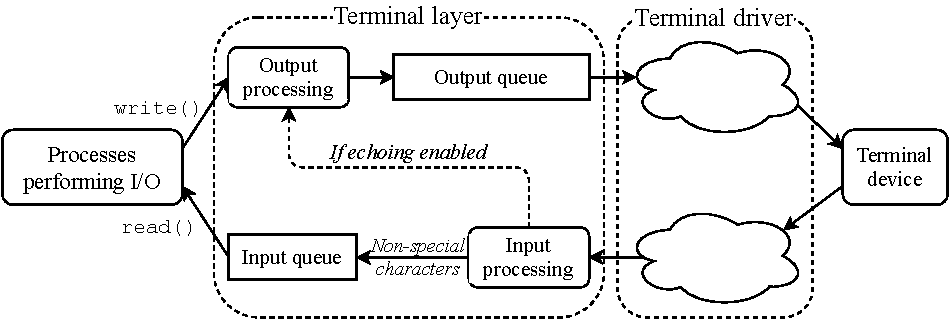
\includegraphics[width=\textwidth, keepaspectratio]{img/term-hilevel-new}
  \caption{A high-level overview of terminal data flow. The clouds in the
    terminal driver symbolize two things: first, the terminal layer is not
    concerned with how the driver processes the characters it receives from the
    hardware or from the the terminal layer. Second, different drivers may
    process characters differently.}
  \label{fig:term-hilevel}
\end{figure}

\subsubsection{Controlling terminals}

A terminal may be designated as the controlling terminal of a session. A session
may have at most one controlling terminal, and a terminal may be the
controlling terminal of at most one session. A process can always access its
controlling terminal (if it has one) by opening the \Verb{/dev/tty} device file.
We define the controlling terminal of a process to be simply the controlling
terminal of that process's session.

When a session is created, it has no controlling terminal. The session leader is
responsible for setting and changing the controlling terminal device, although
the way in which this is done is not specified in the standard.

When the leader of a session terminates, the controlling terminal (if any) is
dissociated from the session. Any processes left in the session can, but don't
need to, have their access to the controlling terminal revoked (see
\cite[Section~11.1.3]{terminal-spec}). For instance, the FreeBSD kernel revokes
access to the controlling terminal (see \cite[Section~8.6, Subsection~``Process
Groups, Sessions, and Terminal Control'']{freebsd-book}) , while the Mimiker
kernel does not. The behaviour found in Mimiker is a conscious design decision
made by the author for the sake of simplicity.

If a controlling terminal disappears from the system (e.g.\ due to the terminal
device no longer being available), the leader of the associated session, is sent
a \Verb{SIGHUP} signal. The signal is sent only to the leader, not to all
processes in the session. Note that the signal is not necessarily fatal, as it
can be caught or ignored by any process.

\subsubsection{Foreground process groups}

Access to the controlling terminal of processes can be controlled using
foreground and background process groups.

A process group may be designated as the foreground process group of its
session's controlling terminal. All other process groups in the session are
background process groups. The foreground process group of a terminal can be set
using the \Verb{tcsetpgrp()}\cite{tcsetpgrp} function. Any process can set the
foreground process group of its controlling terminal, although some restrictions
apply to processes from background process groups. A controlling terminal does
not need to have a foreground process group at all times.

Processes in the foreground process group are allowed to \Verb{read()} and
\Verb{write()} to their controlling terminal. When a process in a background
process group attempts to \Verb{read()} or \Verb{write()} to its controlling
terminal, every process in its process group is sent a \Verb{SIGTTIN} or
\Verb{SIGTTOU} signal respectively. The default effect of both signals is to
stop the target process. In the case of \Verb{write()}, the signal is sent
only if the \Verb{TOSTOP} terminal flag is set. If it is not set, background
processes can write to their controlling terminal without restrictions. The
exact semantics are a bit more nuanced, see \cite[Section~11.1.4]{terminal-spec}.

As a concrete example, when a shell is accepting input from the user, its
process is necessarily in the foreground process group. When the shell starts a
job, the job is usually put in the foreground, so that the user can interact
with it. The shell waits for the foreground job to complete, and then makes its
own process group the foreground process group, so that it can accept the next
command.

The user may make the job run in the background by appending \Verb{&} to the
command. In that case, the shell remains in the foreground process group and
does not wait for the job to complete. As explained earlier, a background job
will be stopped if it tries to accept input from the user.

A background job can be put in the foreground using the \Verb{fg} shell command.
The command simply sets the controlling terminal's foreground process group to
the process group of the target job, continues the target job if it was stopped,
and waits for the new foreground job's termination.

Figure~\ref{fig:proc-hierarchy-tty} presents the process hierarchy from
Figure~\ref{fig:proc-hierarchy}, but now it includes the concepts of controlling
terminals and foreground process groups.

\begin{figure}[h]
  \centering
  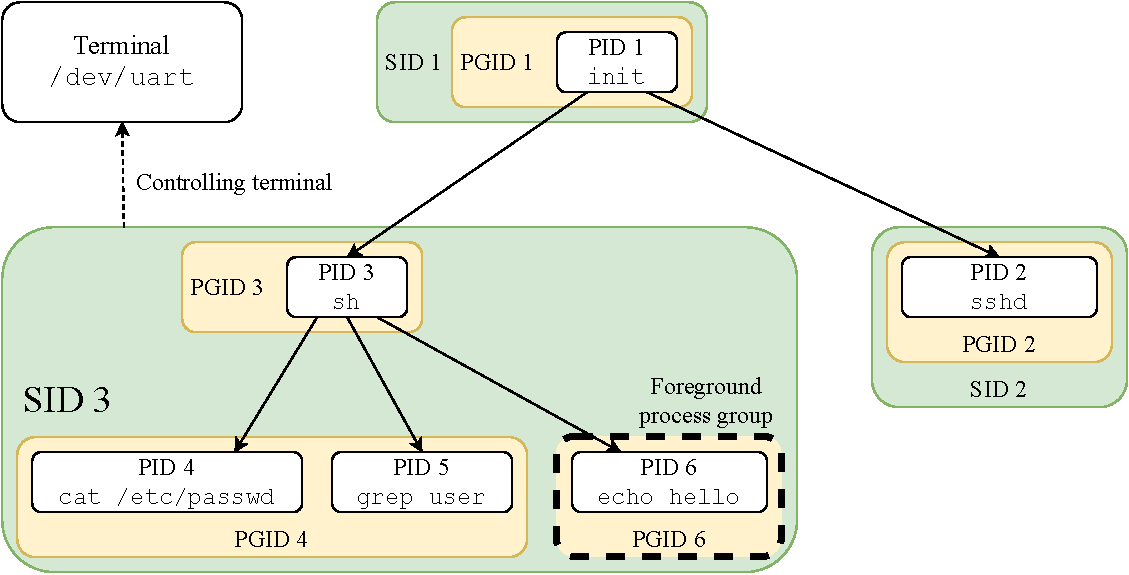
\includegraphics[width=\textwidth, keepaspectratio]{img/proc-hierarchy-tty}
  \caption{Proces hierarchy from figure~\ref{fig:proc-hierarchy} with
    controlling terminals and foreground process groups included. Note that
    sessions 1 and 2 do not have a controlling terminal. The terminal
    \Verb{/dev/uart} is the controlling terminal of session~3. Process group 6
    is the controlling terminal's foreground process group. Once process 6
    terminates, the shell (PID 3) will set the foreground process group to its
    own process group (PGID 3).}\label{fig:proc-hierarchy-tty}
\end{figure}

\subsubsection{Terminal modes and flags}\label{chap:terminal-flags}

Command line applications can be roughly divided into two groups, depending on
how they consume user input:
\begin{itemize}
  \item{One line at a time (\textit{line-oriented}).}
  \item{One character at a time (\textit{character-oriented}).}
\end{itemize}

A shell belongs to the first group, because it accepts a whole command at a
time. Most notably, the user may edit the command before submitting it to the
program by pressing the return key (labelled ``Enter'' on most keyboards).

A text editor like \Verb{vi} belongs to the second group. Each key performs an
action within the editor, such as moving the cursor or inserting text at the
position of the cursor.

In more complex applications, line-oriented input is usually accomplished using
a library such as GNU Readline \cite{readline}. However, POSIX mandates that
basic line-editing functionality is provided by the operating system itself.
Applications may choose whether they want to use this functionality by choosing
the \textit{terminal mode}. Two terminal modes are distinguished:
\textit{canonical} and \textit{non-canonical}, the former providing basic line
editing. The terminal mode has no influence over other aspects of input
processing, such as sending signals in response to certain control characters.

In canonical mode, typed characters are appended to the \textit{line buffer}.
Characters may be erased from the line buffer by typing the special characters
\Verb{VERASE} (which erases the character at the end of the buffer) or
\Verb{VKILL} (which erases the whole buffer). On most systems, the \Verb{VERASE}
character corresponds to the Backspace key on the keyboard, while \Verb{VKILL}
corresponds to Control-U. These special characters are processed by the
operating system and are not forwarded to userspace. Once the user types a
\textit{line-terminating} character (e.g. \Verb{'\n'}, bound to the Return key
on most keyboards), the contents of the line buffer are appended to the input
queue and become available as input to userspace programs.

In non-canonical mode there is no line buffer, and every non-special character
typed by the user is immediately available to userspace programs. The
\Verb{VERASE}, \Verb{VKILL}, and line-terminating characters are no longer
processed in a special way by the OS and appear as input on the terminal.

The terminal mode controls only part of the processing that is performed on
characters coming in. There are many \textit{terminal flags} that can enable
additional character processing on input, as well as output. We will now examine
the data structure that houses almost all terminal settings that can be changed
by userspace programs.

\subsubsection{The \Verb{termios} structure}

For each terminal, almost all of its settings, including the terminal mode, are
stored in a \Verb{termios} structure associated with that terminal. The only
exception is the terminal window size, which isn't a member of the
\texttt{termios} structure and is stored separately. Application code may
examine and modify the contents of this structure using the
\Verb{tcgetattr()}\cite{tcgetattr} and \Verb{tcsetattr()}\cite{tcsetattr}
functions respectively.

The \Verb{termios} structure must contain the following fields:
\begin{itemize}
\item \Verb{c_iflag}: contains flags that control basic terminal input
  handling. Some notable flags are:
  \begin{itemize}
  \item \Verb{ICRNL}: map the \textit{carriage return} (CR, \Verb{'\r'})
    character to the \textit{new line} (NL, \Verb{'\n'}) character on input.
  \item \Verb{BRKINT}: send a \Verb{SIGINT} signal to the foreground process
    group upon detecting a break condition.
  \item \Verb{IGNBRK}: ignore hardware break conditions.
  \item \Verb{INPCK}: enable input parity checking.
  \item \Verb{IGNPAR}: ignore characters with parity errors.
  \end{itemize}
\item \Verb{c_oflag}: contains flags that control terminal output processing.
  Some notable flags are:
  \begin{itemize}
  \item \Verb{OPOST}: enable output processing.
  \item \Verb{ONLCR}: map NL to CR-NL sequence on output.
  \item \Verb{OCRNL}: map CR to NL on output.
  \item \Verb{ONOCR}: do not output CR characters if the cursor is at column
    0.
  \end{itemize}
\item \Verb{c_cflag}: contains flags that control terminal hardware parameters.
  Some notable flags are:
  \begin{itemize}
  \item \Verb{CREAD}: enable hardware receiver.
  \item \Verb{CSIZE}: number of bits transmitted or received per byte (from 5
    to 8).
  \end{itemize}
\item \Verb{c_lflag}: contains flags that control various additional functions.
  Some notable flags are:
  \begin{itemize}
  \item \Verb{ECHO}: enable character echoing. This flag is cleared e.g.\ when the
    user is typing their password.
  \item \Verb{ICANON}: enable canonical mode.
  \item \Verb{ISIG}: send signals in response to certain control characters
    being received.
  \item \Verb{TOSTOP}: send \Verb{SIGTTOU} if a background process tries to
    write to the terminal.
  \end{itemize}
\item \Verb{c_cc}: array defining control character codes. A control character
  can be disabled by setting its code to \Verb{_POSIX_VDISABLE}. Important
  control characters include:
  \begin{itemize}
  \item \Verb{VERASE}: erase the character at the end of the line.
  \item \Verb{VKILL}: erase the whole line.
  \item \Verb{VEOF}: marks the end of input to a program.
  \item \Verb{VINTR}: if the \Verb{ISIG} flag is set, send \Verb{SIGINT}
    to the foreground process group.
  \item \Verb{VSUSP}: if the \Verb{ISIG} flag is set, send \Verb{SIGTSTP}
    (terminal stop signal) to the foreground process group.
  \end{itemize}
\end{itemize}
The current values of terminal flags and control characters can be examined from
the shell using the \Verb{stty} program~\cite{stty}, available on most UNIX-like operating
systems, including Linux. To list the current values of all terminal flags and
control characters for the shell's controlling terminal, use the command:
\begin{quote}
  \Verb{stty -a}
\end{quote}
For the full specification of the \Verb{termios} structure, see~\cite{termios}.

\subsection{Terminals in the Mimiker kernel}\label{chap:mimiker-tty}

We will now describe the implementation of the terminal layer in the Mimiker
kernel.

\subsubsection{Overall design}

The terminal layer provides the abstraction of a terminal to userspace
processes, as well as to the rest of the kernel. It contains code that is
independent of the underlying hardware terminal device. In the subsystem
hierarchy, it sits below the generic file handling layer and above terminal
drivers.

The layer is responsible for character processing, as well as buffering them in
the input and output queues. It includes a mechanism to notify the hardware
terminal driver when new characters arrive in the output queue, as well as when
space becomes available in the input queue.

\subsubsection{Data structures}

\subsubsection*{\Verb{tty_t}}

The \Verb{tty_t} structure encapsulates the hardware-independent state
associated with a single terminal. Among other things, it contains the
\Verb{termios} structure, which houses the terminal's settings.

\begin{listing}[H]
\begin{minted}{c}
typedef enum {
  TF_WAIT_OUT_LOWAT = 0x1,
  TF_WAIT_DRAIN_OUT = 0x2,
  TF_OUT_BUSY = 0x4,
  TF_IN_HIWAT = 0x8,
  TF_DRIVER_DETACHED = 0x10
} tty_flags_t;

typedef struct tty {
  mtx_t t_lock;
  tty_flags_t t_flags;
  ringbuf_t t_inq;
  condvar_t t_incv;
  ringbuf_t t_outq;
  condvar_t t_outcv;
  linebuf_t t_line;
  size_t t_column;
  size_t t_rocol, t_rocount;
  condvar_t t_serialize_cv;
  ttyops_t t_ops;
  struct termios t_termios;
  struct winsize t_winsize;
  pgrp_t *t_pgrp;
  session_t *t_session;
  vnode_t *t_vnode;
  uint32_t t_opencount;
  void *t_data;
} tty_t;
\end{minted}
\caption{\href{https://mimiker.ii.uni.wroc.pl/source/xref/mimiker/include/sys/tty.h?r=ac2bafa1\#62}{\Verb{include/sys/tty.h}: definition of \Verb{tty_t}.}}
\label{lst:tty-t}
\end{listing}

The \Verb{t_lock} mutex synchronizes access to the structure.
\Verb{t_flags} may contain the following flags:
\begin{itemize}
\item \Verb{TF_WAIT_OUT_LOWAT}: a thread is waiting for space to become
  available in the output queue.
\item \Verb{TF_WAIT_DRAIN_OUT}: a thread is waiting for the output queue to
  become empty.
\item \Verb{TF_OUT_BUSY}: a thread is currently writing to this terminal.
  This flag is used to serialize \Verb{write()} calls on the same terminal.
\item \Verb{TF_IN_HIWAT}: the \textit{input high watermark} has been reached.
  The watermark is reached when the terminal driver attempts to insert a
  character into the input queue while it is already full. Once space becomes
  available in the input queue, the hardware terminal driver will be notified.
\item \Verb{TF_DRIVER_DETACHED}: the hardware terminal driver detached from this
  terminal, usually because the terminal device is no longer available. Any
  further I/O on this terminal should return an error.
\end{itemize}

\Verb{t_inq} is a ring buffer storing input coming from the hardware terminal
driver. A ring buffer is a data structure implementing a FIFO queue with a
bounded size. They are a popular in OS kernels thanks to their simplicity and
efficiency. \Verb{read()} calls on the terminal file descriptor receive
characters from this buffer. \Verb{t_incv} is a condition variable used to wait
for input to become available in \Verb{t_inq}.

\Verb{t_outq} is a ring buffer storing characters that should be written out by
the underlying driver. The characters can come from processes writing to the
terminal, or from the input processing stage, where characters can be echoed.
The terminal driver reads characters from this buffer and takes care of
transmitting them. \Verb{t_outcv} is a condition variable used to wait for space
to become available in the output queue or for the queue to become empty.

\Verb{t_line} stores the contents of the line the user is typing in canonical
mode. The type \Verb{linebuf_t} is a structure containing a buffer containing
the line's contents, the current length of the line, and the maximum capacity of
the buffer. The line's contents can be edited by the user. Once the user submits
the line, its contents are copied into \Verb{t_inq}. The contents of
\Verb{t_inq} cannot be changed. In non-canonical mode, \Verb{t_line} is not
used.

\Verb{t_column} keeps track of the position of the terminal cursor. It is
needed to support the \Verb{ONOCR} terminal flag, which forbids sending the
carriage return character when the cursor is at column 0.

The \Verb{t_rocol} and \Verb{t_rocount} fields are needed due to the fact that
the echoed line being typed in by the user can be interleaved with output from
processes, and we only want to let the user erase the characters they typed, not
ones output by processes. The two fields keep track of the longest prefix of the
line that is not interrupted by output from processes.

The \Verb{t_serialize_cv} condition variable is used by processes calling
\Verb{write()} to wait for their turn to access the terminal.

\Verb{t_ops} is a structure containing implementations of terminal driver
operations. There are currently four operations that a driver can supply, but
only one is required:
\begin{listing}[H]
\begin{minted}{c}
typedef void (*t_notify_out_t)(struct tty *);
typedef void (*t_notify_in_t)(struct tty *);
typedef void (*t_notify_active_t)(struct tty *);
typedef void (*t_notify_inactive_t)(struct tty *);

typedef struct {
  t_notify_out_t t_notify_out;
  t_notify_in_t t_notify_in;
  t_notify_active_t t_notify_active;
  t_notify_inactive_t t_notify_inactive;
} ttyops_t;
\end{minted}
\caption{\href{https://mimiker.ii.uni.wroc.pl/source/xref/mimiker/include/sys/tty.h?r=ac2bafa1\#28}{\Verb{include/sys/tty.h}: definition of \Verb{ttyops_t}.}}
\end{listing}
The \Verb{t_notify_out} function notifies the driver that new data has appeared
in the terminal structure's output queue (i.e. \Verb{t_outq}). The driver should
ensure that data from the queue is written out to the terminal device as soon as
possible. It is the only function implemented by both terminal drivers, i.e. the
UART and pseudoterminal drivers.

The \Verb{t_notify_in} function notifies the driver that space has become
available in the input queue (i.e. \Verb{t_inq}).

The \Verb{t_notify_active} function is called when the number of open file
descriptors for the terminal increases from 0 to 1. Predictably,
\Verb{t_notify_inactive} is called when the number of open file descriptors
drops from 1 to 0.

The terminal configuration described in the previous section is stored in the
\Verb{t_termios} field. The terminal window size is stored separately in the
\Verb{t_winsize} field. The \Verb{t_pgrp} field points to the foreground process
group, if any, while \Verb{t_session} points to the session controlled by this
terminal.

\Verb{t_vnode} points to the filesystem node representing the terminal. It is
used to implement the \Verb{/dev/tty} device file, which refers to different
terminals for processes in different sessions. The \Verb{t_opencount} field
keeps track of the number of open file descriptors for the terminal.
\Verb{t_data} is an opaque pointer for the underlying terminal driver to store
its private data.

In addition to the above fields, there are macros convenience macros
\Verb{t_lflag}, \Verb{t_cflag}, \Verb{t_iflag}, \Verb{t_oflag}, and \Verb{t_cc}.
These expand to the corresponding members of the \Verb{t_termios} field. For
instance, \Verb{t_lflag} expands to \Verb{t_termios.c_lflag}.

\subsubsection{Lifecycle of a terminal}

When a terminal driver attaches to a device, it is responsible for creating its
corresponding terminal in the kernel. This involves allocating a new
\Verb{tty_t} structure, setting device-specific fields in that structure (e.g.
\Verb{t_ops}) and creating a special device file referring to the terminal in
the \Verb{/dev} directory of the filesystem.

The \Verb{tty_makedev()} function takes care of creating the special file. When
creating the file, the function supplies \Verb{tty_fileops} to the file-handling
layer as the implementation of file operations. This way, \Verb{read()} and
\Verb{write()} (and other) calls on the file are directed to the terminal layer,
which may in turn call the terminal driver via \Verb{t_ops}.

Once a terminal is created and visible in the filesystem, processes can open and
perform I/O on it.

The process of deleting a terminal begins when the terminal driver detects that
the underlying device is no longer available (e.g. due to a modem disconnect).
The driver then \textit{detaches} itself from the in-kernel terminal structure.
After that happens, processes are no longer able open or perform I/O on the
terminal. Once the last open file descriptor referencing the terminal is closed,
the terminal structure's memory is reclaimed.

\subsubsection{Terminal input}

Processes read data from a terminal by invoking \Verb{read()} on an open
terminal file descriptor. The generic file-handling layer in the kernel then
uses the \Verb{fo_read} function pointer in the structure representing the open
file to call the appropriate function for that particular type of file. In the
case of files representing terminals, the \Verb{fo_read} function pointer is set
to the \Verb{tty_read()} function.

The \Verb{tty_read()} function does very little besides calling
\Verb{tty_do_read()}, which does the actual work of reading characters from the
input queue. Its very slightly simplified source code is presented in
Listing~\ref{lst:tty-do-read}.

\begin{listing}[H]
\begin{minted}{c}
static int tty_do_read(file_t *f, uio_t *uio) {
  tty_t *tty = f->f_data;
  int error = 0;
  uint8_t c;

  WITH_MTX_LOCK (&tty->t_lock) {
@\llabel{f1}@    if (tty_detached(tty))
      return ENXIO;

    while (true) {
@\llabel{f2}@      if ((error = tty_check_background(tty, SIGTTIN)))
        return error;
@\llabel{f3}@      if (tty->t_inq.count > 0)
        break;
@\llabel{f4}@      if ((error = tty_wait(tty, &tty->t_incv)))
        return error;
    }

    if (tty->t_lflag & ICANON) {
      /* In canonical mode, read as many characters as possible,
       * but no more than one line. */
      while (ringbuf_getb(&tty->t_inq, &c)) {
@\llabel{f5}@        if (CCEQ(tty->t_cc[VEOF], c))
          break;
        if ((error = uiomove(&c, 1, uio)))
          break;
@\llabel{f6}@        if (uio->uio_resid == 0)
          break;
        /* Check for end of line. */
@\llabel{f7}@        if (tty_is_break(tty, c))
          break;
      }
    } else {
@\llabel{f8}@      ringbuf_getb(&tty->t_inq, &c);
      error = uiomove(&c, 1, uio);
    }

@\llabel{f9}@    tty_check_in_lowat(tty);
  }

  return error;
}
\end{minted}
\caption{\href{https://mimiker.ii.uni.wroc.pl/source/xref/mimiker/sys/kern/tty.c?r=7a5a999c\#595}{\Verb{kern/tty.c}: simplified definition of \Verb{tty_do_read()}.}}
\label{lst:tty-do-read}
\end{listing}

The \Verb{f} parameter points to a \Verb{file_t} structure representing an open
file. Since the file represents a terminal, the \Verb{f_data} field contains a
pointer to the associated terminal's \Verb{tty_t} structure.

The \Verb{uio_t} structure describes the destination or source buffer (or
buffers) of an I/O operation in the kernel. The \Verb{uio_resid} field contains
the number of remaining bytes to be processed. Its design in the Mimiker kernel
(see file \Verb{include/sys/uio.h}) was inspired by the \Verb{struct uio}
structure found in kernels from the BSD family, see e.g. \cite{uio-man}.

After acquiring the terminal's mutex, we first \ref{f1} check whether the driver
has detached from this terminal. If it has, we cannot do any more I/O on it, so
we return an error. 

The next step is to check whether we are currently allowed to read from the
terminal. As previously mentioned, processes in background process groups are
usually not allowed to read from their controlling terminal. The
\ref{f2} \Verb{tty_check_background()} function determines whether the calling process
can perform I/O on the given terminal. The \Verb{SIGTTIN} argument specifies
that we are trying to read from the terminal. If the function determines that we
are not allowed to continue with the operation, it will return an error code. It
may also send the specified signal (\Verb{SIGTTIN} in this case) to every
process in the calling process's process group.

Next, we \ref{f3} check whether the input queue contains any characters. The
\Verb{read()} system call is blocking (at least by default), so if no data is
available, the calling thread is put to sleep awaiting data. This is why, if the
input queue is empty, we go on to \ref{f4} call \Verb{tty_wait()} to wait on the
\Verb{t_incv} condition variable. The role of the \Verb{tty_wait()} function
will be explained at the end of this section.

Once the \Verb{tty_wait()} function returns \Verb{0}, we must repeat the checks
starting from \ref{f2}, since we may no longer be allowed to read from the
terminal, e.g. because our process group was moved to the background. Repeating
the check at \ref{f1} is not necessary, since \Verb{tty_wait()} does it for us.
The loop continues until we find that there are characters in the input queue.

After breaking out of the loop, we need to decide how to read the characters. In
canonical mode, at most one line can be read in a single \Verb{read()} call. The
\Verb{VEOF} character behaves like a line terminator, but it is special in that
it doesn't get passed to userspace. This is why we check for it at \ref{f5},
before we copy the character read from the input queue to the user buffer. After
copying the character, we \ref{f6} check whether we have filled the user buffer
or \ref{f7} whether the character was an ordinary line terminator. In both
cases, we break out of the read loop.

In non-canonical mode, \ref{f8} exactly one character is read and returned to
userspace. This behaviour is very different from that specified in POSIX (see
\cite[Section~11.1.7]{terminal-spec}), where the semantics of \Verb{read()} in
non-canonical mode depend on the values of the \Verb{VMIN} and \Verb{VTIME}
parameters stored in the \Verb{t_cc} array. The POSIX semantics are considerably
more difficult to implement and provide little to no benefit, since no
applications that have been ported to Mimiker actually use them.

Finally, \ref{f9} the \Verb{tty_check_in_lowat()} function will notify the
driver if the input high watermark had been previously reached and the number of
characters in the input queue has dropped below a certain threshold.

We have covered how characters find their way from the terminal input queue to
the buffer supplied by the reading user process. The question that remains is:
How are characters written into the input queue?

It is the responsibility of the terminal driver to pass characters arriving at
the hardware device to the terminal layer. The driver does this by invoking the
\Verb{tty_input()} function on the terminal structure, supplying the new
character. The function takes care of all input processing and putting
characters into the input queue.

Due to the number of terminal flags affecting input processing, the source code
of the \Verb{tty_input()} function is quite large. For this reason, we will only
take a look at the function's control flow, with many details omitted for the
sake of readability.

\begin{listing}[H]
\begin{minted}{c}
void tty_input(tty_t *tty, uint8_t c) {
  handle IGNCR, ICRNL and INLCR flags;

  if (ISIG flag is set) {
    /* Signal processing */
    if (c is VINTR or VSUSP or VQUIT) {
      send the appropriate signal to the foreground process group;
      return;
    }
  }

  if (ICANON flag is set) {
    /* Line editing */
    if (c is VERASE or VKILL) {
      erase the approriate characters from the line;
      return;
    }

    insert c into the line buffer;
    
    if (c is a line terminator) {
      append the line buffer to the input queue; 
      notify threads waiting on t_incv;
    }
  } else {
    insert c into the input queue;
    notify threads waiting on t_incv;
  }

  if (ECHO flag is set) {
    echo c;
  }
}
\end{minted}
\caption{\href{https://mimiker.ii.uni.wroc.pl/source/xref/mimiker/sys/kern/tty.c?r=7a5a999c\#471}{\Verb{kern/tty.c}: simplified control flow of \Verb{tty_input()}.}}
\end{listing}

The \Verb{t_incv} condition variable is used by reading threads to wait for data
in the input queue. Other than that, the listing is fairly self-explanatory, so
we won't go into detail describing every step.

This is a good moment to take a closer look at the \Verb{tty_wait()} function,
which is used throughout the terminal layer to wait on condition variables. It
performs extra checks to make sure that the terminal driver hasn't detached from
the terminal while the calling thread was sleeping.

\begin{listing}[H]
\begin{minted}{c}
static int tty_wait(tty_t *tty, condvar_t *cv) {
  int error;

@\llabel{p1}@  error = cv_wait_intr(cv, &tty->t_lock);

@\llabel{p2}@  if (tty_detached(tty))
    return ENXIO;

  /* Did we receive a signal while sleeping? */
@\llabel{p3}@  if (error == EINTR)
    return ERESTARTSYS;

  return error;
}

\end{minted}
\caption{\href{https://mimiker.ii.uni.wroc.pl/source/xref/mimiker/sys/kern/tty.c?r=7a5a999c\#192}{\Verb{kern/tty.c}: definition of \Verb{tty_wait()}.}}
\label{lst:tty-wait}
\end{listing}

The function first \ref{p1} sleeps on the given condition variable. Note that it
passes \Verb{&tty->t_lock} as the second argument to \Verb{cv_wait_intr()}, so
the lock on the \Verb{tty} terminal is released before going to sleep. After
being woken up, the \Verb{cv_wait_intr()} function acquires the lock before
returning. However, note that almost anything could have happened to the
terminal while we were sleeping, since we were not holding the terminal's
\Verb{t_lock}. Most importantly, the associated driver might have detached from
the terminal, in which case we must disallow any further I/O. Therefore,
immediately after waking up we \ref{p2} check whether the driver has detached
and return an error code if it has.

Instead of being woken up by another thread signalling the condition variable, it
is also possible that we were woken up by receiving a signal that needs
handling. In other words, our sleep was \textit{interrupted} (that's what the
\Verb{intr} in \Verb{cv_wait_intr() stands for} --- \textit{interruptible}). At
\ref{p3} we check whether our sleep was interrupted by a signal. If it was, we
return \Verb{ERESTARTSYS}, which is a special return value that will cause the
system call to be restarted if it turns out that no signal has been caught.
This special return value is explained in more detail in
Section~\ref{chap:sleep-stop}.

\subsubsection{Terminal output}

Processes write data to a terminal by invoking \Verb{write()} on an open
terminal file descriptor. The kernel in turn calls \Verb{tty_write()} via the
\Verb{fo_write} function pointer to carry out the operation.

\begin{listing}[H]
\begin{minted}{c}
static int tty_write(file_t *f, uio_t *uio) {
  tty_t *tty = f->f_data;
  int error = 0;

  WITH_MTX_LOCK (&tty->t_lock) {
    if (tty_detached(tty))
      return ENXIO;

    if (tty->t_lflag & TOSTOP) {
@\llabel{g1}@      if ((error = tty_check_background(tty, SIGTTOU)))
        return error;
    }

@\llabel{g2}@    while (tty->t_flags & TF_OUT_BUSY)
      if ((error = tty_wait(tty, &tty->t_serialize_cv)))
        return error;
    tty->t_flags |= TF_OUT_BUSY;

    error = tty_do_write(tty, uio);

    tty->t_flags &= ~TF_OUT_BUSY;
    cv_signal(&tty->t_serialize_cv);
  }

  return error;
}
\end{minted}
\caption{\href{https://mimiker.ii.uni.wroc.pl/source/xref/mimiker/sys/kern/tty.c?r=7a5a999c\#796}{\Verb{kern/tty.c}: simplified definition of \Verb{tty_write()}.}}
\label{lst:tty-write}
\end{listing}

The function's primary role is to \ref{g1} check whether we are allowed to
perform the operation using \Verb{tty_check_background()} and to serialize calls
to \Verb{tty_do_write()} by \ref{g2} waiting until the \Verb{TF_OUT_BUSY} flag
is cleared.

The \Verb{tty_do_write()} function is responsible for putting each character in
the supplied buffer into the output queue and notifying the driver.

\begin{listing}[H]
\begin{minted}{c}
static int tty_do_write(tty_t *tty, uio_t *uio) {
  uint8_t c;
  int error = 0;

  while (uio->uio_resid > 0) {
@\llabel{n1}@    if ((error = uiomove(&c, 1, uio)))
      break;
@\llabel{n2}@    if ((error = tty_output_sleep(tty, c)))
      break;
    tty->t_rocount = 0;
  }
@\llabel{n3}@  tty_notify_out(tty);

  return error;
}
\end{minted}
\caption{\href{https://mimiker.ii.uni.wroc.pl/source/xref/mimiker/sys/kern/tty.c?r=7a5a999c\#775}{\Verb{kern/tty.c}: simplified definition of \Verb{tty_do_write()}.}}
\label{lst:tty-do-write}
\end{listing}

The function \ref{n1} reads consecutive characters from the buffer supplied by
the process and \ref{n2} puts them into the output queue one at a time using
\Verb{tty_output_sleep()}. At the end, it \ref{n3} notifies the terminal driver
of new data using \Verb{tty_notify_out()}.

The \Verb{tty_output_sleep()} function puts a single character into the output
queue, sleeping if there is no space available.

\begin{listing}[H]
\begin{minted}{c}
static int tty_output_sleep(tty_t *tty, uint8_t c) {
  int error;
@\llabel{o1}@  while (!tty_output(tty, c)) {
@\llabel{o2}@    tty_notify_out(tty);
    /* tty_notify_out() can synchronously write characters to the device,
     * so it may have written enough characters for us not to need to sleep. */
@\llabel{o3}@    if (tty->t_outq.count < TTY_OUT_LOW_WATER)
      continue;
@\llabel{o4}@    tty->t_flags |= TF_WAIT_OUT_LOWAT;
@\llabel{o5}@    if ((error = tty_wait(tty, &tty->t_outcv)))
      return error;
  }
  return 0;
}
\end{minted}
\caption{\href{https://mimiker.ii.uni.wroc.pl/source/xref/mimiker/sys/kern/tty.c?r=7a5a999c\#760}{\Verb{kern/tty.c}: definition of \Verb{tty_output_sleep()}.}}
\label{lst:tty-output-sleep}
\end{listing}

The function repeatedly \ref{o1} attempts to insert the character into the
output queue using \Verb{tty_output()}, which will return \Verb{false} if there
is no space left in the queue. If that happens, we wait until the number of
characters in the output queue drops below the \textit{output low watermark}.
Before going to sleep, we \ref{o2} notify the terminal driver to make sure that
it will eventually transfer some characters from the output queue, allowing us
to proceed. The driver may transfer the characters \textit{synchronously}, i.e.
directly in the \Verb{tty_notify_out()} function, which is why we must \ref{o3}
check whether the low watermark has already been reached. If it hasn't, we
\ref{o4} set the \Verb{TF_WAIT_OUT_LOWAT} flag to indicate that there is a
thread waiting for space in the output queue, and finally we \ref{o5} go to
sleep on the \Verb{t_outcv} condition variable. The variable will be signalled
by the driver after it makes enough space available in the output queue.

Let us now take a look at the code of the \Verb{tty_output()}, which takes care
of output character processing and putting the characters into the output queue.

\begin{listing}[H]
\begin{minted}{c}
static bool tty_output(tty_t *tty, uint8_t c) {
  int oflag = tty->t_oflag;
  if (!(oflag & OPOST)) {
@\llabel{h1}@    return tty_outq_putc(tty, c);
  }

  uint8_t cb[2];
  cb[0] = c;
@\llabel{h2}@  int ccount = tty_process_out(tty, oflag, cb);
  int col = tty->t_column;

@\llabel{h3}@  if (!tty_outq_write(tty, cb, ccount))
    return false;

@\llabel{h4}@  for (int i = 0; i < ccount; i++) {
    adjust the col variable based on the character class of cb[i];
  }
  tty->t_column = col;
  return true;
}
\end{minted}
\caption{\href{https://mimiker.ii.uni.wroc.pl/source/xref/mimiker/sys/kern/tty.c?r=7a5a999c\#708}{\Verb{kern/tty.c}: simplified definition of \Verb{tty_output()}.}}
\label{lst:tty-write}
\end{listing}

If the \Verb{OPOST} flag isn't set, we skip all output processing and \ref{h1}
write the character directly to the output queue. Otherwise, we \ref{h2} call
\Verb{tty_process_out} to handle \Verb{OCRNL}, \Verb{ONLCR} and \Verb{ONOCR}
terminal flags. During processing, a single character can be converted into two
characters due to the \Verb{ONLCR} flag, which is why we use the \Verb{cb}
buffer to store them, and \Verb{ccount} is the number of resulting characters
after processing. If the input flag \Verb{OXTABS} was implemented (currently it
is not), then a single character could be converted into as many as eight
characters, since if the flag is set, a tab character (\Verb{'\t'}) is converted
into eight spaces.

We then \ref{h3} attempt to write the processed characters to the output queue.
The call to \Verb{tty_outq_write()} will return \Verb{false} if there isn't
enough space in the output queue for the characters. If that's the case, we
return \Verb{false} to indicate failure. 

If we successfully wrote the characters to the output queue, then we need to
adjust the value of the terminal's \Verb{t_column} field, which keeps track of
the column number of the terminal cursor. Each character has a \textit{class},
which determines how it impacts the column number. For instance, the
\Verb{BACKSPACE} class (which contains only the backspace character \Verb{'\b'})
decreases the column number by one, unless the column number is already zero.
We therefore \ref{h4} loop over every character we have written to the output
queue and adjust the column number based on its class.

Finally, we return \Verb{true} to indicate that we have successfully written the
characters to the output queue.

After the characters have been written to the output queue and the terminal
driver has been notified, it is up to the driver to consume characters from the
queue and transmit them to the hardware device. We will examine how this is done
in the case of the UART driver in Section~\ref{chap:tty-uart}. 

\subsubsection{Controlling terminals}

As seen in Section~\ref{chap:sessions}, the controlling terminal for a
session is stored in the \Verb{s_tty} field of \Verb{session_t}. When a
new session is created, its \Verb{s_tty} field is set to \Verb{NULL}.

A terminal becomes the controlling terminal of a session automatically when that
session's leader opens a terminal file. The association happens only when the
session doesn't already have a controlling terminal, and the terminal being
opened isn't associated with any session.

When the session leader process exits, the session loses its controlling
terminal. This is the only way a terminal may become dissociated from its
session.

\subsubsection{Foreground process groups}

The \Verb{t_pgrp} field in the \Verb{tty_t} structure points to the foreground
process group associated with the terminal. Only controlling terminals (i.e.\
ones associated with a session) may have a foreground process group. When a
terminal first becomes associated with a session, its foreground process group
is set to the process group of the session leader.

The \Verb{tcgetpgrp()} and \Verb{tcsetpgrp()} functions are provided by the
standard C library. Their implementations use the \Verb{ioctl()} system call
to perform the required operation.

\Verb{ioctl()} is a very general, catch-all system call that is most commonly
used to provide functionality that is too simple to merit a separate system
call. It takes as arguments a file descriptor, an \textit{opcode} (short for
\textit{operation code}), and a generic argument. The opcode is simply a numeric
value that tells the kernel what operation to perform. The argument's
interpretation depends on the specific opcode. Most opcodes are only valid for
file descriptors of a certain type, e.g.\ ones representing terminals. The
opcodes used for getting and setting the foreground process group are
\Verb{TIOCGPGRP} and \Verb{TIOCSPGRP} respectively.

When the foreground process group becomes empty, the terminal's \Verb{t_pgrp}
field is set to \Verb{NULL}. Thus, a terminal does not need to have a
foreground process group at all times, even if it is associated with a session.

\section{The UART terminal driver}
\label{chap:tty-uart}

The terminal layer delegates the task of transmitting characters over the
hardware device to a \textit{terminal driver}. Currently, the only hardware
supported by the terminal subsystem is UART, a simple serial link. In this
section, we will see how the UART driver interacts with the device-independent
terminal layer.

\subsection{General design}

The driver consists of two main components:
\begin{itemize}
\item A \textit{worker thread} that handles data transfers between the driver
  and the terminal layer.
\item An \textit{interrupt service routine} (ISR) that responds to hardware events
  (e.g. a new character being received).
\end{itemize}

The driver has two internal buffers separate from the terminal layer's input and
output queues: a \textit{transmit} and \textit{receive buffer}. The transmit
buffer holds characters taken from the output queue, while the receive buffer
holds characters waiting to be processed by the \Verb{tty_input()} function.

Actually, the driver does not need to use an intermediate transmit buffer
between the terminal's output buffer and the hardware. It may simply write all
data from the buffer in a single invocation of \Verb{t_notify_out}. In other
words, the driver may output the characters \textit{synchronously}. However,
that would most likely require busy-waiting for the hardware to become ready to
accept data, unnecessarily consuming CPU time. For this reason, an
\textit{asynchronous} approach is taken in this driver.

The worker thread transfers characters from the terminal structure's output
queue to the transmit buffer, and passes characters from the receive buffer to
the terminal layer using the \Verb{tty_input()} function.

The interrupt service routine takes characters from the transmit buffer and
writes them to the appropriate device registers to send them over the UART link.
It also receives characters directly from the hardware and puts them in the
receive buffer.

A good question to ask at this point is: do we even need the worker thread?
Couldn't we instead call \Verb{tty_input()} directly when receiving a character
in the ISR and output characters to the UART directly (i.e. synchronously) in
\Verb{t_notify_out}?

The answer is yes, we do need the worker thread. Calling \Verb{tty_input()}
directly from the ISR would violate the kernel's synchronization rules, as
\Verb{tty_input()} uses mutexes for synchronization, and mutexes cannot be
acquired in an ISR, only spinlocks. A thread context is needed to acquire the
necessary mutex before calling \Verb{tty_input()}. Therefore, even if we
performed output synchronously, we would still need a worker thread to do the
input processing.

The flow of data between the terminal layer's queues, the UART driver's buffers
and the UART device is shown in Figure~\ref{fig:term-hilevel-uart}. In the
figure, different ``agents'' are responsible for different parts of the data
flow, labelled with numbers:
\begin{itemize}
\item The thread executing the \Verb{write()} system call copies the characters
  from the userspace buffer (1), processes them, and puts them in the terminal's
  output queue (2).
\item The UART driver's worker thread transfers characters between the output
  queue and the UART transmit buffer (3) or writes them directly to the UART
  hardware, bypassing the transmit buffer (10). It also takes characters from
  the UART receive buffer and processes them (6). Characters echoed during input
  processing go through output processing (9) and into the output queue (2).
  After input processing, the worker thread puts the characters in the
  terminal's input queue (7).
\item The UART driver's interrupt service routine writes characters from the
  UART transmit buffer to the UART hardware (4) and puts characters received
  from the UART hardware into the receive buffer (5).
\item The thread executing the \Verb{read()} system call copies characters from
  the terminal's input queue to the userspace buffer (8).
\end{itemize}

\begin{figure}[H]
  \centering
  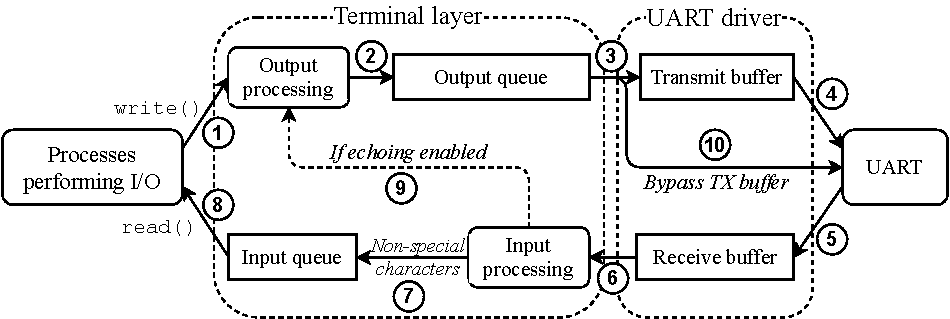
\includegraphics[width=\textwidth, keepaspectratio]{img/term-hilevel-uart-new}
  \caption{Data flow between the terminal layer's queues, the UART driver's
    buffers and the UART device.}
  \label{fig:term-hilevel-uart}
\end{figure}

\subsection{Data structures}

\subsubsection*{\Verb{tty_thread_t}}

The \Verb{tty_thread_t} structure represents a worker thread.
\begin{listing}[H]
\begin{minted}{c}
typedef struct tty_thread {
  thread_t *ttd_thread;
  tty_t *ttd_tty;
  condvar_t ttd_cv;
  uint8_t ttd_flags;
} tty_thread_t;
\end{minted}
\caption{\href{https://mimiker.ii.uni.wroc.pl/source/xref/mimiker/include/sys/uart_tty.h?r=ac2bafa1\#16}{\Verb{include/sys/uart_tty.h}: definition of \Verb{tty_thread_t}.}}
\end{listing}

The \Verb{ttd_thread} field is a pointer to the \Verb{thread_t} structure
representing the thread. The \Verb{ttd_tty} field is the worker thread's
assigned terminal. The \Verb{ttd_cv} condition variable is used by the worker
thread to wait for a signal from the ISR to do some work. The \Verb{ttd_flags}
field is used to communicate what work needs to be done. It can contain the
following flags:
\begin{itemize}
\item \Verb{TTY_THREAD_TXRDY}: The worker thread should transfer characters from
  the terminal layer's output queue to the transmit buffer.
\item \Verb{TTY_THREAD_RXRDY}: The worker thread should transfer characters from
  the receive buffer to the terminal layer using the \Verb{tty_input()}
  function.
\item \Verb{TTY_THREAD_OUTQ_NONEMPTY}: This flag is used as an optimization. It
  tells the ISR whether it should wake up the worker thread to fill the transmit
  buffer. If the flag is cleared, then the terminal layer's output queue is
  empty, so it's unnecessary to wake up the worker to fill the transmit buffer.
  At first, this flag might seem redundant: why not just check how many
  characters are in the terminal's output queue? Notice that holding the
  terminal's mutex is required in order to access its output queue. We need to
  know whether the queue is empty in the ISR, which is not allowed to acquire
  mutexes. Therefore, we use this flag as a workaround, as access to it requires
  holding the UART's \Verb{u_lock} spinlock, which is allowed in an ISR.
\end{itemize}

\subsubsection*{\Verb{uart_state_t}}

The \Verb{uart_state_t} structure encapsulates the UART driver state associated
with a single device.

\begin{listing}[H]
\begin{minted}{c}
typedef struct uart_state {
  spin_t u_lock;
  ringbuf_t u_rx_buf;
  ringbuf_t u_tx_buf;
  tty_thread_t u_ttd;
  void *u_state;
} uart_state_t;
\end{minted}
\caption{\href{https://mimiker.ii.uni.wroc.pl/source/xref/mimiker/include/dev/uart.h?r=2609772a\#44}{\Verb{include/sys/uart.h}: definition of \Verb{uart_state_t}.}}
\end{listing}

The \Verb{u_lock} spinlock protects all fields of the structure, including the
\Verb{u_ttd} field containing the worker thread and its flags. The receive and
transmit buffers are in the \Verb{u_rx_buf} and \Verb{u_tx_buf} fields
respectively. The \Verb{u_state} field holds state specific to the UART hardware
the driver is handling, such as the locations of device registers.

\subsection{UART terminal driver implementation}

Let us now examine the primary components of the UART terminal driver:
\begin{itemize}
\item The driver's implementation of the \Verb{t_notify_out} operation.
\item The worker thread's main loop.
\item The hardware interrupt service routine.
\end{itemize}

\subsubsection{\Verb{uart_tty_notify_out()}}

The \Verb{uart_tty_notify_out()} function is called by the terminal layer
whenever new characters are inserted to the output queue. The function does very
little besides calling \Verb{uart_tty_fill_txbuf()}, which transfers characters
from the output queue to the UART's transmit buffer. Actual output is performed
in the driver's ISR. 

In theory, we do not need to call \Verb{uart_tty_fill_txbuf()} here. Instead, we
could signal the worker thread to do the work for us. However, that would incur
extra overhead due to synchronization and context switching. In order to avoid
it, we try not to involve the worker in moving characters from the output queue
to the transmit buffer.

\begin{listing}[H]
\begin{minted}{c}
static void uart_tty_fill_txbuf(device_t *dev) {
  uart_state_t *uart = dev->state;
  tty_t *tty = uart->u_ttd.ttd_tty;
  uint8_t byte;

  while (true) {
    SCOPED_SPIN_LOCK(&uart->u_lock);
@\llabel{i1}@    uart_tty_try_bypass_txbuf(dev);
@\llabel{i2}@    if (ringbuf_full(&uart->u_tx_buf) || !ringbuf_getb(&tty->t_outq, &byte)) {
@\llabel{i3}@      if (!ringbuf_empty(&uart->u_tx_buf))
        uart_tx_enable(dev);
@\llabel{i4}@      tty_set_outq_nonempty_flag(&uart->u_ttd);
      break;
    }
@\llabel{i5}@    tty_set_outq_nonempty_flag(&uart->u_ttd);
@\llabel{i6}@    ringbuf_putb(&uart->u_tx_buf, byte);
  }
@\llabel{i7}@  tty_getc_done(tty);
}
\end{minted}
\caption{\href{https://mimiker.ii.uni.wroc.pl/source/xref/mimiker/sys/kern/uart_tty.c?r=2609772a\#39}{\Verb{sys/kern/uart_tty.c}: definition of \Verb{uart_tty_fill_txbuf()}.}}
\label{lst:uart-tty-fill-txbuf}
\end{listing}

The function consists of a loop that moves characters from the \Verb{tty}
terminal's output queue to the transmit buffer. However, before transferring any
characters, we \ref{i1} try to bypass the transmit buffer entirely, transmitting
characters directly from the output queue to the hardware. If we didn't try to
bypass the transmit buffer, writing a single character to the terminal would
always wake up the worker thread, which incurs extra overhead due to context
switches. Such single-character writes are common, for example, when echoing
characters typed by the user.

The next step is to \ref{i2} check whether the transmit buffer is full or the
output queue is empty. If neither condition is true, then we can \ref{i6}
transfer a single character. Before that, we \ref{i5} update the
\Verb{TTY_THREAD_OUTQ_NONEMPTY} flag. We then return to the beginning of the
loop.

If either condition at \ref{i2} is true, we can no longer transfer any
characters. In that case, if there are characters in the transmit buffer, we
\ref{i3} tell the hardware to send an interrupt whenever it's ready to accept
data. That way, the ISR will be called and it will move characters from the
transmit buffer to the hardware. We then \ref{i5} update the
\Verb{TTY_THREAD_OUTQ_NONEMPTY} flag before breaking out of the loop.

The last step in the function is \ref{i7} calling \Verb{tty_getc_done()}. In the
case of terminal drivers that output characters asynchronously, the driver is
responsible for waking up threads waiting for space in the terminal's output
queue. This is done by calling the \Verb{tty_getc_done()} function after moving
characters from the output queue. This function simply checks whether the number
of characters in the output buffer has fallen below some threshold. If it has,
it wakes up all waiters waiting on the \Verb{t_outcv} condition variable.

\subsubsection{The worker thread loop}

The worker thread loop is essential to the operation of the UART driver. It is
the link connecting the driver's transmit and receive buffers with the terminal
layer's output and input queues.

\begin{listing}[H]
\begin{minted}{c}
static void uart_tty_thread(void *arg) {
  device_t *dev = arg;
  uart_state_t *uart = dev->state;
  tty_thread_t *ttd = &uart->u_ttd;
  tty_t *tty = ttd->ttd_tty;
  uint8_t work, byte;

  while (true) {
    WITH_SPIN_LOCK (&uart->u_lock) {
      /* Sleep until there's work for us to do. */
@\llabel{j1}@      while ((work = ttd->ttd_flags & TTY_THREAD_WORK_MASK) == 0)
        cv_wait(&ttd->ttd_cv, &uart->u_lock);
      ttd->ttd_flags &= ~TTY_THREAD_WORK_MASK;
    }
    WITH_MTX_LOCK (&tty->t_lock) {
      if (work & TTY_THREAD_RXRDY) {
@\llabel{j2}@        while (uart_getb_lock(uart, &byte))
@\llabel{j3}@          if (!tty_input(tty, byte))
            klog("dropped character %hhx", byte);
      }
      if (work & TTY_THREAD_TXRDY)
@\llabel{j4}@        uart_tty_fill_txbuf(dev);
    }
  }
}
\end{minted}
\caption{\href{https://mimiker.ii.uni.wroc.pl/source/xref/mimiker/sys/kern/uart_tty.c?r=2609772a\#75}{\Verb{sys/kern/uart_tty.c}: definition of \Verb{uart_tty_thread()}.}}
\end{listing}

The first step in the loop is to \ref{j1} wait until the ISR gives us a signal
to do some work by setting at least one of the flags contained in
\Verb{TTY_THREAD_WORK_MASK}, i.e. \Verb{TTY_THREAD_RXRDY} or
\Verb{TTY_THREAD_TXRDY}.

Once we get a signal, we check what kind of work needs to be done. If
the \Verb{TTY_THREAD_RXRDY} flag is set, we \ref{j2} read characters from the
receive buffer and \ref{j3} pass them to the terminal layer using the
\Verb{tty_input()} function. If the \Verb{TTY_THREAD_TXRDY} flag is set, we
\ref{j4} move characters from the terminal's output queue to the transmit buffer
using the \Verb{uart_tty_fill_txbuf()} function.

\subsubsection{The interrupt service routine}

The UART driver's interrupt service routine responds to two kinds of hardware events:
\begin{itemize}
\item A character has been received (``RX Ready'').
\item The hardware is ready to accept a new character (``TX Ready'').
\end{itemize}

The ISR performs the actual transmission of characters in the transmit buffer.
The hardware signals that is ready to accept a character via an interrupt. The
ISR then takes one character from the transmit buffer and writes it to a
hardware register. When the transmit buffer runs out of characters, the ISR
wakes up a worker thread that copies characters from the terminal's output
queue into the transmit buffer.

\begin{listing}[H]
\begin{minted}{c}
intr_filter_t uart_intr(void *data) {
  device_t *dev = data;
  uart_state_t *uart = dev->state;
  tty_thread_t *ttd = &uart->u_ttd;

  WITH_SPIN_LOCK (&uart->u_lock) {
@\llabel{k1}@    if (uart_rx_ready(dev)) {
@\llabel{k2}@      (void)ringbuf_putb(&uart->u_rx_buf, uart_getc(dev));
@\llabel{k3}@      ttd->ttd_flags |= TTY_THREAD_RXRDY;
      cv_signal(&ttd->ttd_cv);
    }

@\llabel{k4}@    if (uart_tx_ready(dev)) {
      uint8_t byte;
@\llabel{k5}@      while (uart_tx_ready(dev) && ringbuf_getb(&uart->u_tx_buf, &byte))
        uart_putc(dev, byte);
@\llabel{k6}@      if (ringbuf_empty(&uart->u_tx_buf)) {
@\llabel{k7}@        if (ttd->ttd_flags & TTY_THREAD_OUTQ_NONEMPTY) {
@\llabel{k8}@          ttd->ttd_flags |= TTY_THREAD_TXRDY;
          cv_signal(&ttd->ttd_cv);
        }
@\llabel{k9}@        uart_tx_disable(dev);
      }
    }
  }
}
\end{minted}
\caption{\href{https://mimiker.ii.uni.wroc.pl/source/xref/mimiker/sys/drv/uart.c?r=2609772a\#18}{\Verb{sys/kern/uart.c}: definition of \Verb{uart_intr()}.}}
\end{listing}

If \ref{k1} a character has been received by the hardware, we \ref{k2} put it
into the receive buffer and \ref{k3} signal the worker thread to pass the
character to the terminal layer.

If \ref{k4} the hardware is ready to accept a new character, we \ref{k5} try to
transmit as many characters from the transmit buffer as possible, hence the
while loop. After that, if \ref{k6} we have emptied the transmit buffer, we
\ref{k8} signal the worker thread to move some characters into the transmit
buffer, but only if \ref{k7} the terminal's output queue is not empty. If the
transmit buffer is empty, we also \ref{k9} prevent the hardware from reporting
TX ready interrupts, as we can't do anything about them until the worker thread
puts some data in the transmit buffer. The \Verb{uart_tty_fill_txbuf()} function
takes care of enabling the interrupt, see Listing~\ref{lst:uart-tty-fill-txbuf}.

\section{Pseudoterminals}

Apart from embedded systems and debugging, character-based communication with
the user over a serial link is becoming increasingly rare. Commodity desktop
systems use a \textit{graphical} shell instead of a text-based one. However,
text-based interaction with the system is still possible thanks to
\textit{terminal emulators}.

A terminal emulator is a program that provides an illusion of a terminal device
to processes and the user. On the user side, the emulator displays a graphical
window with contents of the emulated terminal window. On the process side, it
exposes a terminal file that behaves in the same way as a normal terminal file
would. Processes can open it and perform I/O on it. The terminal emulator plays
the role of the hardware device: it translates the user's keystrokes into
characters that are then made available as input to the processes reading from
the emulated terminal. It also reads the characters output by processes and
displays them in the emulated terminal window.

The OS facility which allows for the emulation of a terminal device in software
is called a \textit{pseudoterminal}. A terminal emulator is far from the only
use case for pseudoterminals. Programs like \Verb{sshd} (an SSH server) or
\Verb{script} (which records an interactive terminal session into a file) also
use pseudoterminals as a basic component. We will now take a look at how POSIX
specifies their operation.

\subsection{POSIX pseudoterminals}

A pseudoterminal consists of a pair of devices: a \textit{master device} and a
\textit{slave device}. The slave device is exposed to processes as a normal
terminal. The master device is used to emulate the terminal device exposed by
the slave.

The master and slave devices are linked together: everything written to the
master device is processed by the terminal layer as though it came from a
hardware device, and is made available as input to processes reading from the
slave device. Similarly, everything written to the slave device goes through
output processing in the terminal layer and appears as input to processes
reading from the master device. The flow of data between master and slave
devices is shown in Figure~\ref{fig:term-hilevel-pty}.

\begin{figure}[h]
  \centering
  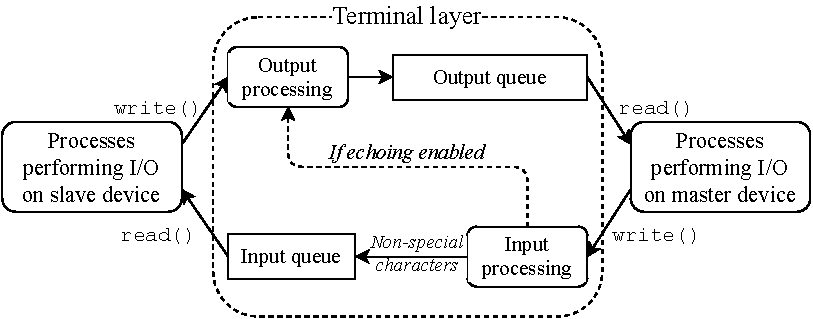
\includegraphics[width=\textwidth, keepaspectratio]{img/term-hilevel-pty}
  \caption{Data flow between the pseudoterminal master and slave devices, with
    the terminal layer's queues acting as intermediate buffers.}
  \label{fig:term-hilevel-pty}
\end{figure}

A new pseudoterminal can be created using the
\Verb{posix_openpt()}\cite{posix-openpt} function. It returns an open file
descriptor to the master device of a pseudoterminal. Note that the master device
isn't exposed in the filesystem: initially only the the process that created the
pseudoterminal has access to the master device (although it can duplicate and
transfer the file descriptor to another process).

Once a pseudoterminal is created, its slave device is accessible via the
filesystem. The slave device files are usually inside the \Verb{/dev/pts}
directory. The file path of the slave device corresponding to a particular
master device can be retrieved using the \Verb{ptsname()}\cite{ptsname}
function.

The slave device is available as long as the master device file is open. Once
the last master device file descriptor is closed, the slave device disappears
from the filesystem, and the effect is as though the emulated terminal device
was disconnected from the system. Any subsequent I/O operation on the slave
device fails with an error code.

\subsection{Pseudoterminals in the Mimiker kernel}

The implementation of pseudoterminals in the Mimiker kernel is relatively
simple, as most of the logic is already implemented in the terminal layer. All
master device logic is implemented as a terminal driver and plugs into the
terminal layer in the same way as the UART driver.

\subsubsection{Data structures}

\subsubsection*{\Verb{pty_t}}

There is very little state associated with a pseudoterminal, as most of the
state is managed by the terminal layer. The \Verb{pty_t} structure contains
pseudoterminal-specific state.
\begin{listing}[H]
\begin{minted}{c}
typedef struct {
  atomic_int pt_number;
  condvar_t pt_incv;
  condvar_t pt_outcv;
} pty_t;
\end{minted}
\caption{\href{https://mimiker.ii.uni.wroc.pl/source/xref/mimiker/sys/kern/pty.c?r=60656d5d\#26}{\Verb{sys/kern/pty.c}: definition of \Verb{pty_t}.}}
\end{listing}

The \Verb{pt_number} field is a unique number identifying the pseudoterminal.
The number determines the filesystem path under which the slave device is
available. For instance, if \Verb{pt_number} is equal to 3, the slave device's
path is \Verb{/dev/pts/3}.

The \Verb{pt_incv} condition variable is used by master-side readers to wait for
data to become available in the slave terminal's \textbf{output} queue, while
the \Verb{pt_outcv} condition variable is used by master-side writers to wait
for space to become available in the slave terminal device's \textbf{input}
queue.

\subsubsection{Master-side input}

Processes read from the master device of a pseudoterminal using the
\Verb{read()} system call, which inside the kernel uses the \Verb{fo_read}
function pointer to call the appropriate implementation. In the case of master
device files, that function pointer points to \Verb{pty_read()}. Let us examine
how it operates.

\begin{listing}[H]
\begin{minted}{c}
static int pty_read(file_t *f, uio_t *uio) {
  tty_t *tty = f->f_data;
  pty_t *pty = tty->t_data;
  int error;

  SCOPED_MTX_LOCK(&tty->t_lock);

  /* Wait until there is at least one byte of data. */
@\llabel{l1}@  while (ringbuf_empty(&tty->t_outq)) {
@\llabel{l2}@    if (!tty_opened(tty))
      return 0;
@\llabel{l3}@    if (cv_wait_intr(&pty->pt_incv, &tty->t_lock))
      return ERESTARTSYS;
  }

@\llabel{l4}@  error = ringbuf_read(&tty->t_outq, uio);
@\llabel{l5}@  tty_getc_done(tty);

  return error;
}
\end{minted}
\caption{\href{https://mimiker.ii.uni.wroc.pl/source/xref/mimiker/sys/kern/pty.c?r=60656d5d\#49}{\Verb{sys/kern/pty.c}: definition of \Verb{pty_read()}.}}
\end{listing}

The function first \ref{l1} loops until there is some data in the corresponding
slave terminal's output queue. If \ref{l2} the slave terminal isn't opened by
any processes, we return without reading anything. Otherwise, we \ref{l3} wait
on the pseudoterminal's \Verb{pt_incv} condition variable. If our sleep got
interrupted by a signal, we return an error code of \Verb{ERESTARTSYS}.

The \Verb{pt_incv} condition variable is signaled when new data arrives in the
slave terminal's output queue. Recall from Section~\ref{chap:mimiker-tty}
that the \Verb{t_notify_out} function is called when new characters are added to
the output queue. This function's implementation is supplied by the driver, so
in our case, the function simply wakes up all threads waiting on the
\Verb{pt_incv} condition variable:
\begin{listing}[H]
\begin{minted}{c}
static void pty_notify_out(tty_t *tty) {
  pty_t *pty = tty->t_data;
  /* Notify PTY readers: input is available. */
  cv_broadcast(&pty->pt_incv);
}
\end{minted}
\caption{\href{https://mimiker.ii.uni.wroc.pl/source/xref/mimiker/sys/kern/pty.c?r=60656d5d\#200}{\Verb{sys/kern/pty.c}: definition of \Verb{pty_notify_out()}.}}
\end{listing}

Once we get past the loop, we know that there is data available in the output
queue, so we \ref{l4} read the data into the buffer supplied by the reading
process. The interface of the terminal layer requires us to call
\Verb{tty_getc_done()} after consuming characters from the output queue, so
at \ref{l5} we do just that.

\subsubsection{Master-side output}

Writing to the master device is accomplished in the kernel using the
\Verb{pty_write()} function, which hooks into the \Verb{fo_write} operation in
the generic file-handling layer.

\begin{listing}[H]
\begin{minted}{c}
static int pty_write(file_t *f, uio_t *uio) {
  tty_t *tty = f->f_data;
  pty_t *pty = tty->t_data;
  int error = 0;
  uint8_t c;
  uiostate_t save;

  SCOPED_MTX_LOCK(&tty->t_lock);

@\llabel{m1}@  while (uio->uio_resid > 0) {
@\llabel{m2}@    uio_save(uio, &save);
@\llabel{m3}@    if ((error = uiomove(&c, 1, uio)))
      break;
@\llabel{m4}@    if ((error = pty_putc_sleep(tty, pty, c))) {
@\llabel{m5}@      uio_restore(uio, &save);
      break;
    }
  }

  return error;
}
\end{minted}
\caption{\href{https://mimiker.ii.uni.wroc.pl/source/xref/mimiker/sys/kern/pty.c?r=60656d5d\#93}{\Verb{sys/kern/pty.c}: definition of \Verb{pty_write()}.}}
\end{listing}

The function \ref{m1} loops as long as there are character left to write in the
buffer supplied by the calling process. Before reading the actual character,
\ref{m2} the current status of the I/O operation is saved. We then \ref{m3} read
the character to be written from the userspace buffer and \ref{m4} write it to
the slave terminal's input queue using the \Verb{pty_putc_sleep()} function,
which sleeps on the \Verb{pt_outcv} condition variable if there's no space in
the input queue, and also returns an error if the slave terminal isn't opened by
any processes. Once there's space in the input queue, the \Verb{t_notify_in}
function pointer is invoked, which in our case points to \Verb{pty_notify_in}:
\begin{listing}[H]
\begin{minted}{c}
static void pty_notify_in(tty_t *tty) {
  pty_t *pty = tty->t_data;
  /* Notify PTY writers: there is space in the slave TTY's input queue. */
  cv_broadcast(&pty->pt_outcv);
}
\end{minted}
\caption{\href{https://mimiker.ii.uni.wroc.pl/source/xref/mimiker/sys/kern/pty.c?r=60656d5d\#206}{\Verb{sys/kern/pty.c}: definition of \Verb{pty_notify_in()}.}}
\end{listing}

If the \Verb{pty_putc_sleep()} function fails, we must roll back the read of the
character at \ref{m3}, since we failed to properly consume it. To do that, we
\ref{m5} restore the previously saved state of the I/O operation. After rolling
back, we break out of the loop and return with an error code.

\chapter{Implementation Challenges}

In order to properly implement terminal and job control support in the Mimiker
kernel, many seemingly unrelated issues needed to be resolved. Some of them were
unimplemented features, while others concerned more fundamental design choices
in the kernel. This chapter describes a number of interesting issues that arose,
and how they have been resolved.

This first issue concerns the way stop signals (e.g. \Verb{SIGSTOP}) interact
with threads that are sleeping interruptibly. The second one arose when trying
to reconcile the existing locking rules with the terminal subsystem's
requirements. The last challenge described involves working around Mimiker's
lack of \Verb{poll()}\cite{poll} and \Verb{select()}\cite{select} functionality
when porting the \Verb{tetris} program.

\section{Interruptible sleep and stop signals}\label{chap:sleep-stop}

When a process performs certain I/O operations (e.g. reading from a terminal),
if the data isn't immediately available, the calling thread will \textit{sleep}
(i.e. suspend execution in the kernel) awaiting the data. Two kinds of sleep are
usually distinguished: \textit{interruptible} and \textit{uninterruptible}.
Interruptible sleep is used in case of I/O that may take an arbitrarily long
time to complete, as is the case when reading from a terminal --- there is no
guarantee that data will eventually arrive. Uninterruptible sleep is used when
the event being awaited is expected to occur within a short time, for instance
during disk I/O.

When a thread sleeping interruptibly receives a signal for which it has
registered a handler, it is resumed so that it can handle the signal: the
thread's sleep has been \textit{interrupted}.

There are two things that can happen after a thread has its sleep interrupted by
a signal, depending on the value of the handler's \Verb{SA_RESTART} flag, whose
value is set when installing a signal handler via
\Verb{sigaction()}\cite{sigaction}:
\begin{itemize}
\item If the flag is set, the interrupted system call is restarted.
\item If the flag is not set, the interrupted system call returns to userspace,
  usually with an error code of \Verb{EINTR}.
\end{itemize}

When a thread receives a stop signal (e.g. \Verb{SIGSTOP}) with a default
disposition\footnote{Note that \Verb{SIGSTOP}'s disposition cannot be changed
  from the default one, see Section~\ref{chap:signals}.}, its execution should
be immediately stopped. Once the thread is resumed using \Verb{SIGCONT},
assuming the \Verb{SIGCONT} signal had no registered handler, according to POSIX
\cite[Section~2.4.4]{general-spec}, the thread should resume at the point it was
stopped. This means that the reception of a \Verb{SIGSTOP} signal followed by
\Verb{SIGCONT} should usually be imperceptible to userspace processes.

In most kernels, signals are usually handled whenever a thread returns from the
kernel to userspace. The set of pending signals for the current thread is
checked, and if a signal which should be delivered is found, it is delivered
either by killing or stopping the thread, or arranging for the signal handler to
be called. Having a single point where signals are handled is beneficial from an
architectural standpoint, as it introduces the smallest possible amount of
complexity, making it easier to understand.

However, what should happen when a stop signal is being sent to a thread that is
sleeping interruptibly? Should it be stopped \textit{while} it is sleeping and
remain sleeping when it is resumed? Or should its sleep be interrupted, making
the interrupted thread continue execution to the userspace boundary, where it
will handle the stop signal itself? Note that in the second case, the system
call that was interrupted must be restarted in order to maintain the illusion
that execution has been resumed at the point it was stopped.

The first approach is implemented in the FreeBSD kernel. It has the advantage of
being somewhat more true to the specification, as the stopped thread will
continue at exactly the point it was stopped. However, there are some drawbacks
to this approach:
\begin{itemize}
\item It introduces additional logic to handle sending a stop signal to a thread
  that is sleeping interruptibly.
\item Signals are no longer always processed at the kernel-userspace boundary:
  stop signals can also be processed when a thread is going to sleep.
\item A thread sleeping interruptibly can be indefinitely prevented from waking
  up by sending it a stop signal. This could potentially be exploited to perform
  denial of service attacks on certain components of the system. For instance, a
  thread writing to a terminal may sleep (interruptibly) on a condition variable
  while having exclusive access to that terminal. If a stop signal is sent to
  that thread while it is sleeping, it won't relinquish its exclusive access
  until it is resumed\footnote{This was an actual bug in the FreeBSD kernel
    found by the author, see\\
    \url{https://bugs.freebsd.org/bugzilla/show_bug.cgi?id=255816}}. A malicious
  program could use this technique to prevent all other processes from writing
  to a terminal.
\end{itemize}
The curious reader can read the relevant FreeBSD (version 13.0) source code: the
\href{https://github.com/freebsd/freebsd-src/blob/releng/13.0/sys/kern/kern_sig.c#L2522}{\Verb{sig_suspend_threads()}}
function found in \Verb{sys/kern/kern_sig.c}\footnote{The FreeBSD source code is
  available at \url{https://github.com/freebsd/freebsd-src}.} is responsible for
stopping the threads of a process. It is called when sending the process a stop
signal.

The second approach, used in the Linux kernel, avoids the drawbacks of the first
approach:
\begin{itemize}
\item Sending a stop signal to a thread that is sleeping interruptibly is done
  in the same way as sending any other signal: if the signal isn't blocked or
  ignored, the receiving thread's sleep is interrupted and the signal is handled
  at the userspace boundary.
\item Signals are processed in one spot: if a thread detects a pending stop
  signal when it is about to go to sleep, it won't go to sleep, and instead
  report to the caller that a signal needs to be handled.
\item Since threads can stop only at the userspace boundary, they can't hold any
  exclusive kernel resource (such as exclusive access to a terminal) when
  stopping.
\end{itemize}

When implementing stop signals in the Mimiker kernel, a choice had to be made
about which approach to choose. The second approach seems conceptually simpler
and avoids the pitfalls of the first one, which is why it was chosen. Let us now
get into more details about how it works.

In the following discussion, a signal is considered \textit{caught} only if its
handler is executed. Therefore, if a thread is stopped using \Verb{SIGSTOP} and
resumed using \Verb{SIGCONT}, assuming \Verb{SIGCONT} had no associated handler,
then no signal was caught. According to this definition, a signal with a default
disposition cannot be caught.

When a thread that is about to go to sleep inside a system call detects a
pending signal, it returns a special error code that specifies under what
circumstances the system call should be restarted:
\begin{itemize}
\item \Verb{ERESTARTSYS}: restart the system call if and only if no signal was
  caught or the caught signal's handler has the \Verb{SA_RESTART} flag set. 
\item \Verb{ERESTARTNOHAND}: restart the system call if and only if no signal
  was caught.
\end{itemize}
Consequently, if a system call returns \Verb{ERESTARTSYS} or
\Verb{ERESTARTNOHAND}, and the only signals handled at the userspace boundary
are \Verb{SIGSTOP} followed by \Verb{SIGCONT} (without a handler), then the
system call will be restarted in the same way it would be if there were no
signals to handle at all.

For an example of how the \Verb{ERESTARTSYS} error code is used in the Linux
kernel, see line 2238 of file
\href{https://elixir.bootlin.com/linux/v5.12.4/source/drivers/tty/n_tty.c#L2238}{\Verb{drivers/tty/n_tty.c}}\footnote{The
  Linux kernel source code is available at \url{https://elixir.bootlin.com/linux/v5.12.4/source}.}
in Linux 5.12.4. Before sleeping, the \Verb{n_tty_read()} function checks for
pending signals and returns \Verb{-ERESTARTSYS} if a signal is pending.

Linux defines two more error codes like this, but at the time of writing they
are not needed to implement any system call in the Mimiker kernel, so they have
not been included:
\begin{itemize}
\item \Verb{ERESTARTNOINTR}: always restart the system call.
\item \Verb{ERESTART_RESTARTBLOCK}: like \Verb{ERESTARTSYS}, except when
  restarting, the interrupted system call is replaced with
  \Verb{restart_syscall()}\cite{restart-syscall}, which adjusts time-related
  parameters (e.g. timeout duration in the case of \Verb{poll()}) before
  restarting the original system call.
\end{itemize}
These error codes may be imported into Mimiker in the future, as more
functionality finds its way into the kernel. The definition of all four special
error codes can be found in the Linux kernel source code (version 5.12.4) in
\href{https://elixir.bootlin.com/linux/v5.12.4/source/include/linux/errno.h}{\Verb{include/linux/errno.h}}.

To illustrate exactly how the Linux approach works when adapted for the Mimiker
kernel, let's trace what happens in Mimiker when a thread sleeping inside the
\Verb{tty_wait()} function is sent a \Verb{SIGSTOP} signal:
\begin{enumerate}
\item In \Verb{sig_kill()}, the thread sending the signal calls
  \Verb{sleepq_abort()} on the sleeping thread, interrupting its sleep (see
  Listing~\ref{lst:sig-kill}).
\item The \Verb{cv_wait_sig()} function called by the sleeping thread returns
  \Verb{EINTR}, indicating the sleep was interrupted.
\item The \Verb{tty_wait()} function converts the \Verb{EINTR} error code to
  \Verb{ERESTARTSYS} (see Listing~\ref{lst:tty-wait}).
\item The \Verb{ERESTARTSYS} error code is propagated through the call stack. If
  the interrupted thread had previously gained exclusive access to the terminal
  in \Verb{tty_write()}, it relinquishes it during this step (see
  Listing~\ref{lst:tty-write}).
\item Before returning to userspace, in \Verb{on_user_exc_leave()} (see
  Listing~\ref{lst:on-user-exc-leave}), the \Verb{sig_check()} function checks
  for pending signals (see Listing~\ref{lst:sig-check}). Signals that should
  stop or kill the receiving process are handled immediately inside
  \Verb{sig_check()}. In our case the only pending signal is \Verb{SIGSTOP}, so
  this is where the thread is stopped.
\item After being resumed via \Verb{SIGCONT}, \Verb{sig_check()} checks for
  pending signals once again. The return value from \Verb{sig_check()} indicates
  whether there are any pending signals with a registered handler. Let's assume
  that no new signals apart from \Verb{SIGCONT} arrived while the thread was
  stopped, and that the \Verb{SIGCONT} has no registered handler, so the return
  value from \Verb{sig_check()} indicates that no signals need to be caught.
\item The return value from \Verb{sig_check()}, along with the system call
  return value (\Verb{ERESTARTSYS} in our case), is passed to
  \Verb{set_syscall_retval()}. This function handles the special return codes
  and arranges for the system call to be restarted if needed. According to the
  semantics of \Verb{ERESTARTSYS}, since no signal is caught, the system call is
  arranged to be restarted by appropriately modifying the userspace thread's
  context.
\item Upon return from the kernel to userspace, the \Verb{write()} system call
  is immediately restarted.
\end{enumerate}

In conclusion, the Linux approach to handling stop signals and interruptible
sleep is a good fit for the Mimiker kernel due to its simplicity. While its
implementation required introducing support for restarting system calls, that
turned out not to be a big problem.

\section{Refinement of locking rules}\label{chap:locking-rules}

As explained in Section~\ref{chap:locking-intro}, locking primitives such as
mutexes are used to synchronize concurrent accesses to members of data
structures that are shared between threads. When using these locking primitives,
care must be taken to prevent \textit{deadlocks}. A deadlock occurs when a group
of two or more threads is stuck, with each thread in the group waiting for a
resource that is held by another thread in the group.

The simplest example of a deadlock is when two threads each attempt to acquire
two mutexes: \Verb{mtx_a} and \Verb{mtx_b}, with thread 1 acquiring the mutexes
in a different order than thread 2. Listing~\ref{lst:deadlock} shows example
code for the threads.
\begin{listing}[h]
\begin{multicols}{2}\centering
Thread 1
\begin{minted}{c}
void thread1(void) {
  mtx_lock(mtx_a);
  mtx_lock(mtx_b);
  /* ... */
  mtx_unlock(mtx_b);
  mtx_unlock(mtx_a);
}
\end{minted}
Thread 2
\begin{minted}{c}
void thread2(void) {
  mtx_lock(mtx_b);
  mtx_lock(mtx_a);
  /* ... */
  mtx_unlock(mtx_a);
  mtx_unlock(mtx_b);
}
\end{minted}
\end{multicols}
\caption{Example code of two threads acquiring mutexes in different orders.}
\label{lst:deadlock}
\end{listing}

Consider the following sequence of events:
\begin{enumerate}
\item Thread 1 acquires \Verb{mtx_a};
\item Thread 2 acquires \Verb{mtx_b};
\item Thread 1 attempts to acquire \Verb{mtx_b} and blocks, since it is already
  held by thread 2;
\item Thread 2 attempts to acquire \Verb{mtx_a} and blocks, since it is already
  held by thread 1.
\end{enumerate}
Clearly, neither thread can proceed, since each thread is waiting for a lock
that is held by the other thread. Hence, we have a deadlock.

One of the most common ways to prevent such deadlocks, employed e.g.\ by FreeBSD
\cite[Section~4.3, Subsection ``Deadlock Prevention'']{freebsd-book} is to
impose an \textit{ordering} on the locks and require that locks are always
acquired according to that ordering. For instance, if we imposed an ordering
that placed \Verb{mtx_a} before \Verb{mtx_b}, it would be illegal to acquire
\Verb{mtx_a} while holding \Verb{mtx_b}. If a thread wanted to acquire both
mutexes, it would need to acquire \Verb{mtx_a} first and then \Verb{mtx_b}.
Thus, the two threads from the example would acquire the two mutexes in the same
ordering, preventing a deadlock from happening.

The Mimiker kernel tries to avoid deadlocks using this method. Whenever multiple
locks are acquired, they are acquired according to an informally defined
ordering. During the integration of the terminal subsystem with other subsystems
of the kernel (e.g. signal handling), the per-terminal
\Verb{t_lock}\footnote{The per-terminal \Verb{t_lock} mutex synchronizes
  accesses to all mutable members of the \Verb{tty_t} structure, see e.g.\
  Listing~\ref{lst:tty-do-write}.} embedded in the \Verb{tty_t} structure had to
be placed somewhere in the lock ordering. This posed some problems, as the
following example illustrates.

Consider what happens when a session leader terminates. If the session has a
controlling terminal, and the terminal has a foreground process group, then
every process in the foreground process group should receive a \Verb{SIGHUP}
signal. In order to access a process's session structure and its controlling
terminal, the \Verb{all_proc_mtx}\footnote{The global \Verb{all_proc_mtx} mutex
  synchronizes accesses to process-tree structures such as process groups and
  sessions, see e.g.\ Listing~\ref{lst:pgrp-enter}.} mutex must be held. In
order to examine a terminal's foreground process group, the terminal's
\Verb{t_lock} mutex must be held. Therefore, \Verb{all_proc_mtx} must be
acquired first in order to look up the controlling terminal, and then
\Verb{t_lock} must be acquired to examine the foreground process group. This
places \Verb{all_proc_mtx} before \Verb{t_lock} in the lock ordering.

After looking up the foreground process group, we might need to send a signal to
each process in the group using the \Verb{sig_pgkill()} function. This function
requires both \Verb{all_proc_mtx} and the target process group's
\Verb{pg_lock}\footnote{The per-process-group \Verb{pg_lock} mutex synchronizes
  accesses to the group's list of member processes, see e.g.\
  Listing~\ref{lst:-pgrp-enter}.} to be held by the caller. This implies that
\Verb{pg_lock} comes after \Verb{t_lock} and \Verb{all_proc_mtx} in the
ordering.

Now that we have established that \Verb{all_proc_mtx} $<$ \Verb{t_lock} $<$
\Verb{pg_lock}, let's look at what needs to happen during terminal input
processing. If the \Verb{ISIG} terminal flag is set, we must send a signal to
every process in the foreground process group in response to certain control
characters. Understandably, character processing happens while holding
\Verb{t_lock}, so that other threads can't change the terminal settings in the
middle of processing. In order to send a signal to the foreground process group,
we must acquire \Verb{all_proc_mtx} and the group's \Verb{pg_lock}. However,
note that acquiring \Verb{all_proc_mtx} while holding \Verb{t_lock} would
violate the ordering!

Several bad solutions quickly come to mind:
\begin{itemize}
\item Require callers of \Verb{tty_input()} to hold \Verb{all_proc_mtx}.\\
  This is bad, because \Verb{all_proc_mtx} is only needed when sending a signal,
  which happens rarely during terminal input processing. Processing of normal
  characters should not bear the cost of synchronization that is needed only in
  exceptional cases.
\item When a signal needs to be sent, drop \Verb{t_lock}, and then acquire
  \Verb{all_proc_mtx}, \Verb{t_lock} and the foreground process group's
  \Verb{pg_lock}.\\
  This might work, but requires some extra precautions.
  First of all, the terminal device might disappear while we are not holding
  \Verb{t_lock}. Secondly, dropping \Verb{t_lock} would lead to headaches for
  callers of \Verb{tty_input()}, which might rely on holding \Verb{t_lock} for
  their own synchronization purposes.
\end{itemize} 

A semi-reasonable solution is to delegate sending the signal to another thread.
This is the approach used in the NetBSD kernel. This approach is actually
\textit{necessary} in the case of NetBSD, as the terminal layer there uses
spinlocks for synchronization, not mutexes, and sending a signal requires
holding a mutex. Since it is illegal to acquire a mutex while holding a
spinlock, delegating the job to a thread is a necessity.

We chose not to follow NetBSD's approach and instead follow the approach found
in the FreeBSD kernel, where it is possible to send a signal to a process group
while holding a terminal's mutex. That's because the locking requirements of the
function used to send signals in FreeBSD are less strict compared to the Mimiker
kernel. We therefore relaxed the locking requirements of the \Verb{sig_kill()}
function, so that it no longer requires \Verb{all_proc_mtx} to be held by the
caller. This was not a trivial task. To understand why, we need to understand
why \Verb{sig_kill()} required \Verb{all_proc_mtx} in the first place.

A parent may be waiting for a child process's state to change using the
\Verb{waitpid()} function. Resuming a process using the \Verb{SIGCONT} signal
counts as a state change. Therefore, the parent of a stopped process receiving a
\Verb{SIGCONT} signal must be notified of the state change. This notification
happens inside the \Verb{sig_kill()} function. The code of the \Verb{wait4()}
system call (which implements the \Verb{waitpid()} POSIX function) used
\Verb{all_proc_mtx} to synchronize with \Verb{sig_kill()}, so if we were to
remove \Verb{all_proc_mtx} from \Verb{sig_kill()}, we would also need to adjust
the \Verb{wait4()} system call's code.

Another complication is that in order to notify the parent, we need to access
the \Verb{p_parent} field of the process receiving the signal. Since this field
is mutable (when a process terminates, it changes its children's \Verb{p_parent}
pointer to another process), accesses to were synchronized using
\Verb{all_proc_mtx}. This requirement also needed to be changed.

The first issue was resolved by using the parent process's \Verb{p_lock} to
synchronize the parent thread with the thread sending the signal. The
\Verb{PF_CHILD_STATE_CHANGED} flag is set in the parent process to tell it that
a child process's state has changed.

The second issue was resolved by changing the locking rules around the
\Verb{p_parent} field of \Verb{proc_t}. The field is now protected by
\textit{two} locks: the process's \Verb{p_lock} and \Verb{all_proc_mtx}. In
order to read the field's value, holding either lock is sufficient. However, in
order to change the value, \textit{both} locks must be held. Since in
\Verb{sig_kill()}  we're only reading the value of \Verb{p_parent}, holding the
target process's \Verb{p_lock} is enough.

While the two issues are now resolved, another problem arises as a result: in
order to notify the parent of the target process's state change, we must acquire
the parent's \Verb{p_lock} \textit{while} holding its child's \Verb{p_lock}.
This used to be forbidden by the locking rules. However, note that we can safely
acquire the parent's mutex if we enforce the following rule:
\begin{quote}
  The \Verb{p_lock} of the parent of a process \Verb{p} may be acquired while
  holding the \Verb{p_lock} of \Verb{p}, but not the other way around.
\end{quote}
Since the process hierarchy forms a tree, there are no cycles, so it is
impossible for a deadlock to occur. We could extend this rule to arbitrary
ancestors instead of just the parent, but currently it does not bring any
additional benefits.

With these adjustments in place, the \Verb{sig_kill()} function no longer
requires \Verb{all_proc_mtx} to be held by the caller, and it's possible to send
a signal to the foreground process group directly from within \Verb{tty_input()}.

\section{Porting \Verb{tetris} to Mimiker}

With the terminal subsystem in place, Mimiker needed an application that would
showcase its capabilities, as well as test them. The well-known game of Tetris
seemed to be a good fit. The NetBSD operating system includes the game in its
sources. It is written in a very simple and portable way, making it a good
candidate for porting to the Mimiker OS. However, there were several challenge
along the way, which will be described in this section.

\subsection{The \Verb{terminfo} library}

NetBSD's \Verb{tetris} program uses advanced terminal features, such as moving
the cursor to arbitrary positions on the screen and coloured output. These
features are implemented using \textit{escape codes}: special character
sequences which are interpreted by the terminal device or terminal emulator.
There is a standard set of ANSI escape
codes\footnote{\url{https://en.wikipedia.org/wiki/ANSI_escape_code}}. For
instance, in order to clear the entire screen on a terminal device supporting
the ANSI escape codes, a program would output the sequence \Verb{^[[2J}, where
\Verb{^[} stands for the \textit{escape} character, whose ASCII code is
\Verb{0x1B}.

Some terminal devices and terminal emulators do not strictly conform to the ANSI
escape code standard. They may implement extra functionality using custom escape
codes, or use different escape codes for functionality that is part of the
standard. This is clearly a problem when trying to write programs that use
advanced terminal features, as supporting all the different escape codes quickly
becomes a pain. This is where the \Verb{terminfo}\cite{libterminfo} library, or
simply \Verb{libterminfo}, comes in to save the day.

The \Verb{terminfo} library provides a portable way of accessing
terminal-related information, such as escape codes. To this end, the library
makes use of a database of information about various specific terminal device
models or terminal emulators. This database is often called the \Verb{terminfo}
database. For instance, on the author's Linux system, the database is located at
\Verb{/usr/lib/terminfo}. When a program using \Verb{libterminfo} wants to e.g.
clear the screen, it would call a library function to get the proper escape code
for the specific terminal device being used. The \Verb{TERM} environment
specifies the model of the terminal device being used.

Since the \Verb{tetris} program uses the \Verb{terminfo} library to handle
escape codes, the library needed to be ported to Mimiker, which was not
especially difficult. Below is a summary of the steps taken to port
\Verb{libterminfo} to Mimiker:
\begin{itemize}
\item Import missing \Verb{libc} functionality from NetBSD (e.g. \Verb{cdb}
  database handling functions).
\item Modify the library's build process to use GNU \Verb{gperf} instead of
  NetBSD's \Verb{nbperf} to generate perfect hashing functions.
\item Add terminal descriptions for several terminal models: \Verb{xterm},
  \Verb{xterm-256color}, \Verb{xterm-direct}, \Verb{vt100}, and \Verb{vt220}.
\item Set the \Verb{TERM} environment variable to a sensible default value (i.e.
  \Verb{xterm}) in the shell's startup script. \Verb{xterm} is a good default
  choice, since it is an old terminal emulator, and most modern emulators are
  compatible with it.
\end{itemize} 

\subsection{Working around lack of \Verb{select()}/\Verb{poll()}}

The biggest issue with porting \Verb{tetris} to Mimiker was how the game handles
user input. Naturally, \Verb{tetris} is an interactive game, so whenever a
character is typed by the user, the game reacts immediately, updating its state
and redrawing the screen. Besides that, the piece that is falling from the top
is periodically lowered, regardless of user input. Therefore, when reading input
from the terminal, some sort of timeout must be used, so that the game doesn't
block indefinitely if the user doesn't press any keys.

In its original form found in NetBSD sources, the \Verb{poll()}\cite{poll}
system call is used to wait for user input with a timeout. Unfortunately, at the
time of writing the Mimiker kernel does not implement the \Verb{poll()} system
call or any other system calls with similar functionality, such as
\Verb{select()}\cite{select}. To make the game work, some workaround had to be
put in place.

Thankfully, there is a viable workaround that uses the \Verb{SIGALRM} signal and
the \Verb{setitimer()}\cite{setitimer} function. The \Verb{setitimer()} function
sets up a \textit{timer} for the calling process. When the timer expires, the
process receives a \Verb{SIGALRM} signal. We can use the timer and the signal as
a timeout mechanism.

Suppose we want to read input from the terminal with a timeout of one second.
First, we set up a handler for the \Verb{SIGALRM} signal that doesn't do
anything. Next, we set a timer to expire one second in the future using the
\Verb{setitmer()} function, and call the \Verb{read()} function to read input
from the terminal. The \Verb{read()} function will sleep awaiting input if none
is available. However, thanks to the timer, it will sleep for at most one
second, since after one second a \Verb{SIGALRM} signal will interrupt the sleep.
If the sleep is interrupted by a signal, the \Verb{read()} function will return
an error code of \Verb{EINTR}, which lets us know that the timeout has expired.
If the \Verb{read()} function returns without an error, which means that input
arrived before the timeout, then we disable the timer.

It is worth repeating that this is a workaround, not a solution. There are some
edge cases that can pose problems. For example, if the timer expires before
calling \Verb{read()}, the \Verb{read()} function will not be interrupted. This
can be remedied by making the timer periodic. 

Funnily enough, this workaround (which works around missing functionality in
Mimiker) itself required functionality that was missing, namely the
\Verb{setitimer()} and \Verb{getitimer()} functions. The functions'
corresponding system calls with the same names had to be implemented in the
kernel from scratch. This required some modifications to the kernel's
\textit{callout} facility, which is used to arrange for functions to be called
at a specified point in time. Overall, the changes required to implement timers
amounted to about 300 lines of code.

With the missing functionality in place, the workaround worked without issues,
and \Verb{tetris} is fully playable on the Mimiker OS. Figure~\ref{fig:tetris}
is a screenshot of \Verb{tetris} running under Mimiker on an emulated MIPS Malta
board.

\begin{figure}[h]
  \centering
  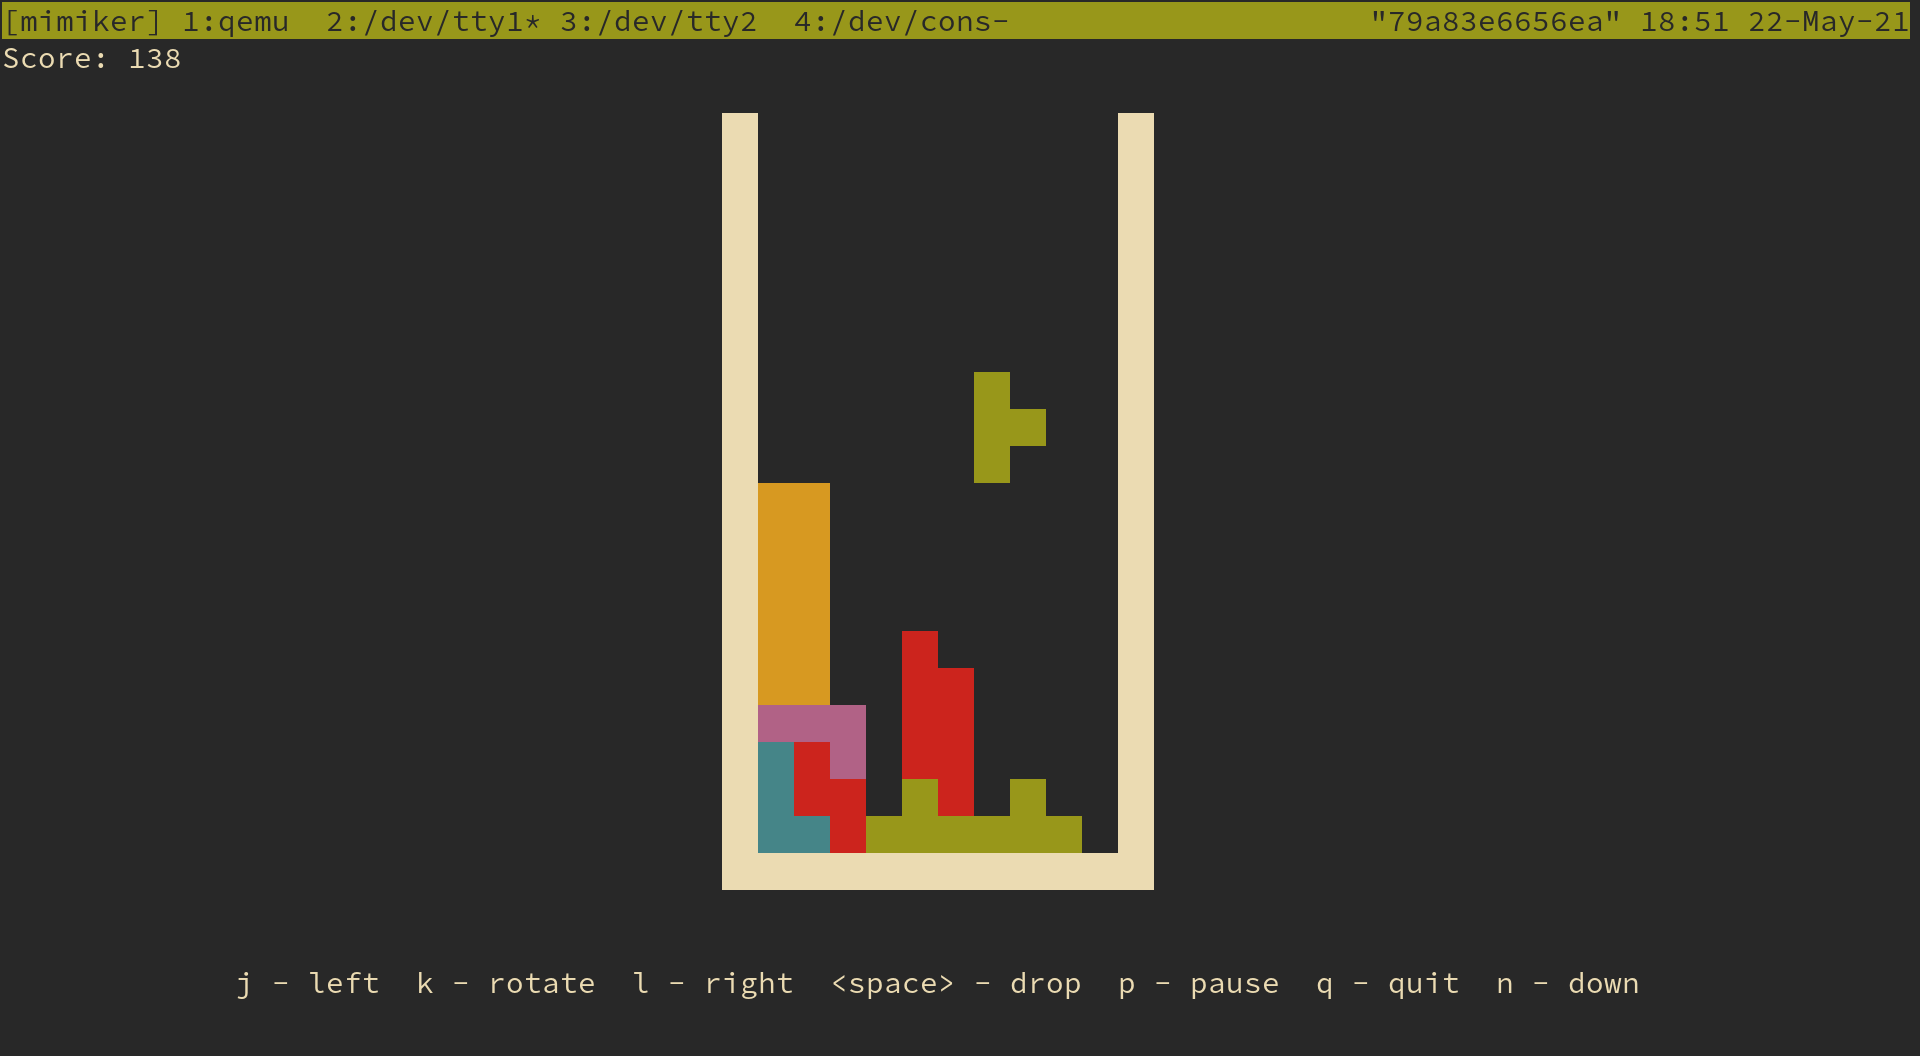
\includegraphics[width=\textwidth, keepaspectratio]{img/tetris}
  \caption{Screenshot of \Verb{tetris} running under Mimiker.}
  \label{fig:tetris}
\end{figure}
\chapter{Conclusion, future work, and usage instructions}

In this chapter, the author's contributions to the Mimiker OS and elsewhere are
first summarized. After that, we lay out notable differences between the POSIX
specification and the implementation described in this thesis. The differences
are usually due to unimplemented features, which provides suggestions for future
work. Finally, we provide instructions on how to compile and run the Mimiker OS,
as well as test some use cases enabled by proper support for job control and the
terminal subsystem.

\section{Summary of contributions}
\subsection*{Mimiker source code}
Below is a summary of the author's code contributions to the Mimiker OS made
as part of the overall implementation effort described in this thesis:
\subsubsection*{Job control}
\begin{itemize}
\item Implementation of process stopping and continuing via signals.\\
  Most important functions:
  \begin{itemize}
  \item \Verb{sys/kern/proc.c}: \Verb{proc_stop()}, \Verb{proc_continue()}
  \item \Verb{sys/kern/signal.c}: \Verb{sig_kill()}, \Verb{sig_check()}
  \end{itemize}
\item Adding support to the \Verb{wait4()} system call for waiting for child
  processes to be stopped or continued.\\
  Most important functions:
  \begin{itemize}
  \item \Verb{sys/kern/proc.c}: \Verb{do_waitpid()}, \Verb{proc_wakeup_parent()}
  \end{itemize}
\item Implementation of POSIX sessions and the \Verb{setsid()} system call.\\
  Most important functions:
  \begin{itemize}
  \item \Verb{sys/kern/proc.c}: \Verb{session_enter()}, \Verb{session_leave()}
  \end{itemize}
\item Expansion of the \Verb{setpgid()} system call's functionality.\\
  Most important functions:
  \begin{itemize}
  \item \Verb{sys/kern/proc.c}: \Verb{pgrp_enter()}
  \end{itemize}
\item Implementation of orphaned process group detection.\\
  Most important functions:
  \begin{itemize}
  \item \Verb{sys/kern/proc.c}: \Verb{pgrp_jobc_leave()}, \Verb{pgrp_jobc_enter()}
  \end{itemize}
\end{itemize}
\subsubsection*{Terminal subsystem}
\begin{itemize}
\item Terminal layer: \Verb{sys/kern/tty.c}
\item UART terminal driver: \Verb{sys/kern/uart_tty.c}, \Verb{sys/drv/uart.c}\\
  Note: the version originally written by the author only supported the UART
  found on the MIPS Malta development board. The code was later adapted by Paweł
  Jasiak to be independent of any specific UART device.
\item Pseudoterminals: \Verb{sys/kern/pty.c}
\end{itemize}
\subsubsection*{Signal handling}
\begin{itemize}
\item Implementation of the \Verb{sigprocmask()} and \Verb{sigsuspend()} system
  calls.\\
  Most important functions:
  \begin{itemize}
  \item \Verb{sys/kern/signal.c}: \Verb{do_sigprocmask()}, \Verb{do_sigsuspend()}
  \end{itemize}
\item Adding support for the \Verb{sa_mask} field in the \Verb{sigaction()}
  system call.\\
  Most important functions:
  \begin{itemize}
  \item \Verb{sys/kern/signal.c}: \Verb{sig_post()}, \Verb{sig_return()}
  \end{itemize}
\item Adding support for the \Verb{SA_RESTART} flag in the \Verb{sigaction()}
  system call and implementation of system call restarting.\\
  Most important functions:
  \begin{itemize}
  \item \Verb{sys/kern/exception.c}: \Verb{on_user_exc_leave()}, \Verb{set_syscall_retval()}
  \end{itemize}
\end{itemize}
\subsubsection*{Ported programs and libraries}
\begin{itemize}
\item \Verb{atto}: minimal \Verb{emacs}-like text editor.
\item \Verb{script}: records terminal input and output into a file.
\item \Verb{libterminfo}: terminal information library.
\item \Verb{tetris}
\end{itemize}
\subsubsection*{Miscellaneous}
\begin{itemize}
\item Management of PIDs, PGIDs and SIDs using hash tables.
\item Extension of the \Verb{devfs} filesystem to allow for removing device nodes.
\item Implementation of \Verb{setitimer()} and \Verb{getitimer()} system calls.
\end{itemize}

\subsection*{Other contributions}
When reading FreeBSD source code, the author found and reported 3 bugs in the
FreeBSD kernel:
\begin{itemize}
\item Bug 250701 - ``Race condition between \Verb{tty_wait_background()} and
    \Verb{doenterpgrp()}''\\
  \url{https://bugs.freebsd.org/bugzilla/show_bug.cgi?id=250701}
\item Bug 251915 - ``TOCTOU race between \Verb{tty_signal_sessleader()} and
  \Verb{killjobc()}''\\
  \url{https://bugs.freebsd.org/bugzilla/show_bug.cgi?id=251915}
\item Bug 255816 - ``tty: Potential DoS on terminal writes by stopping thread inside \Verb{ttydisc_write()}''\\
  \url{https://bugs.freebsd.org/bugzilla/show_bug.cgi?id=255816}
\end{itemize}
All the bugs have been fixed, with the last fix being committed to the
\Verb{main} branch on the 18th of May, 2021.

\section{Future work}

In this section, we provide several possible directions for future work in the
area of job control and the terminal subsystem in the Mimiker OS. The first two
suggestions stem from unimplemented POSIX features. The third one concerns a
behaviour in Mimiker that differs significantly from other, more popular
UNIX-like operating systems. The last suggestion is a general improvement that
would help greatly in porting advanced applications with a text-based user
interface.

\subsubsection*{Unimplemented terminal settings}

The description of the \Verb{termios} structure found in
Section~\ref{chap:posix-terminals} omits many flags which are part of the
specification, but are not used by most terminal-based applications. Many of
them control various properties of the hardware terminal or handling of
transmission errors. Implementing these may be necessary in order to handle real
UART hardware, as opposed to emulated UARTs. Additionally, changing the
\textit{baud rate} (i.e. transmission speed) using \Verb{cfsetispeed()} and
\Verb{cfsetispeed()} functions is not implemented. Below is a summary of
unimplemented terminal settings. The complete specification of terminal settings
can be found in \cite{terminal-spec}.

\begin{itemize}
  \item Parity error handling: \Verb{IGNPAR}, \Verb{INPCK}, \Verb{PARMRK},
    \Verb{PARENB}, \Verb{PARODD}.
  \item Break condition handling: \Verb{BRKINT}, \Verb{IGNBRK}.
  \item Flow control: \Verb{IXANY}, \Verb{IXOFF}, \Verb{IXON}.
  \item Hardware parameters: \Verb{CREAD}, \Verb{CSIZE}, \Verb{CSTOPB}.
\end{itemize}

\subsubsection*{Non-canonical mode \Verb{read()} semantics}

The current implementation of \Verb{tty_do_read()} (see
Listing~\ref{lst:tty-do-read}) unconditionally reads a single character at a
time in non-canonical mode, which does not conform to the specification found in
\cite[Section~11.1.7]{terminal-spec}. In POSIX, the semantics of reading from a
terminal in non-canonical mode can be controlled using the \Verb{MIN} and
\Verb{TIME} parameters, whose values are stored at indices \Verb{VMIN} and
\Verb{VTIME} in the \Verb{c_cc} array found in the \Verb{termios} structure.
Simplifying a bit, the \Verb{TIME} parameter specifies the maximum time the
\Verb{read()} function should wait for a character, and \Verb{MIN} specifies the
minimum number of characters that should be read. For the precise semantics, we
refer the reader to the specification.

\subsubsection*{Revocation of access to controlling terminal after termination
  of session leader}

As explained in Section~\ref{chap:posix-terminals}, when the leader of a session
terminates, the remaining processes in the session may, but do not need to, have
their access to the controlling terminal revoked. The Mimiker kernel currently
does not revoke access to the controlling terminal, as doing it well would
require adding a general file access revocation mechanism, which is fairly
difficult. Adding such a mechanism to the kernel would help bring Mimiker's
behaviour in this area more in line with other modern UNIX-like OSes.

\subsubsection*{Porting the \Verb{curses} library}

In order to port \Verb{tetris} to the Mimiker OS, the \Verb{terminfo} library,
which abstracts the different capabilities and escape codes used by different
terminals, had to be ported as well. This was an important step towards enabling
support for all terminal-based applications, but there is still one crucial
component missing.

Many advanced applications and games with a text-based interface make use of the
\Verb{curses} library. It builds upon the \Verb{terminfo} library to provide
GUI-like building blocks, such as windows or scrollable lists. The \Verb{curses}
library found in NetBSD is considerably larger than \Verb{terminfo} in terms of
lines of code, making it more challenging to port to Mimiker. Having a working
\Verb{curses} library in Mimiker would be a big step towards supporting
applications and games with impressive text-based interfaces.

\section{Compilation and usage instructions}
This section presents step-by-step instructions on how to compile and run
Mimiker, as well as some shell commands that showcase the functionality
implemented by the author. The \Verb{git} and \Verb{docker} programs are assumed
to be installed on the reader's system.

\subsection*{Compiling Mimiker}

\begin{enumerate}
\item Get the source code.\\
  The following command will download the Mimiker sources into the \Verb{mimiker}
  subdirectory of the current working directory:\\
  \Verb{git clone --depth 1 https://github.com/cahirwpz/mimiker}
\item Download the development environment.\\
  Most Mimiker developers use the Mimiker
  server\footnote{\Verb{mimiker.ii.uni.wroc.pl}} to compile and run their code.
  However, access to the server requires an account, which the reader is assumed
  to not have. While the project provides
  instructions\footnote{\url{https://github.com/cahirwpz/mimiker/blob/master/README.md}}
  on how to install the software required to compile Mimiker, the procedure is
  quite cumbersome. For this reason, the author has prepared a Docker container
  with all the software needed to compile and run Mimiker on an emulated
  machine. The following command downloads the container:
  \Verb{docker pull jpiecuch96/mimiker-dev}\\
\item Run a shell inside the development environment.\vspace{0.5em}\\
\begin{BVerbatim}
docker run --rm -it -u 1000 -v $PWD/mimiker:/mimiker -w /mimiker \
  jpiecuch96/mimiker-dev bash
\end{BVerbatim}
  \\
  Note: this command should be run in the directory containing the
  \Verb{mimiker} subdirectory. Also, the reader's user ID is assumed to be 1000
  (which is the case on most systems).\\
\item Compile Mimiker.\\
  Run the following command in the shell inside the development
    environment:\\
  \Verb{make -j$(nproc)}\\
  If the command fails for whatever reason, try running it again without the
  \Verb{-j} option.
\end{enumerate}

\subsection*{Running Mimiker}

To run a shell inside Mimiker, run the following command in the shell
inside the development environment:\\
\Verb{./launch init=/bin/ksh}\\
This should open a \Verb{tmux} session with the \Verb{ksh} shell running in the
active window. We can now run various commands inside Mimiker.

\subsection*{Terminal commands}

This section presents some shell commands that make use of Mimiker's job
control capabilities or the terminal subsystem. Naturally, all commands listed
in this section should be run in a shell inside Mimiker.

\subsubsection*{Terminal access control based on background process groups}

\begin{enumerate}
\item List current terminal settings:\\
  \Verb{stty -a}\\
  The output contains \Verb{-tostop}, which indicates that the \Verb{TOSTOP}
  flag is not set. This means that a process in a background process group
  should be able to write to the terminal.
\item Check that both background and foreground processes can write to the
  terminal:\\
  \Verb{echo background & echo foreground}\\
  Both \Verb{background} and \Verb{foreground} will be output.
\item Check that background processes are not allowed to read from the terminal:\\
  \Verb{cat &}\\
  The \Verb{cat} program tries to read from the terminal, but since it is in a
  background process group, the attempt results in it being stopped by a
  \Verb{SIGTTIN} signal. This can be verified by running the \Verb{jobs}
  command, which will show the stopped process. It can be brought into the
  foreground using the \Verb{fg} command, after which it can be terminated by
  typing \Verb{^C} (Control-C).
\item Set the \Verb{TOSTOP} terminal flag:\\
  \Verb{stty tostop}
\item Check that background processes are not allowed to write to the terminal:
  \Verb{echo background & echo foreground}\\
  This time, only \Verb{foreground} will be output. Running the \Verb{jobs}
  command will reveal that the background process was stopped upon trying to
  write to the terminal. If we bring it into the foreground using \Verb{fg}, 
  \Verb{background} will be output.
\end{enumerate}

\subsubsection*{Recording a terminal session with \Verb{script}}

The \Verb{script} program uses pseudoterminals to record the output of all
programs in a terminal session. It can record the output to a plaintext file,
or it can also record the timestamp of each output event, making it possible to
play back the session exactly as it was recorded.

\begin{enumerate}
\item Change into the \Verb{/tmp} directory:\\
  \Verb{cd /tmp}
\item To record into a plaintext file, just use the command:\\
  \Verb{script}
\item Now type some commands, for instance:\\
  \Verb{echo one && echo two}
\item Type \Verb{^D} (Control-D) to end the recorded terminal session.
\item The plaintext file with the recording is at \Verb{/tmp/typescript}:\\
  \Verb{cat typescript}
\item To record a session with timestamps, use the command:\\
  \Verb{script -r}\\
  To play it back, use:\\
  \Verb{script -pq typescript}
\end{enumerate}

\subsubsection*{Playing \Verb{tetris}}

To play \Verb{tetris}, type the \Verb{tetris} command in the shell.

\bibliography{bibliography}
\bibliographystyle{myplain}
\end{document}
